%%%%%%%%%%%%%%%%%%%%%%%%%%%%%%%%%%%%%%%%%%%%%%%%%%%%%%%%%%%%%%%%%%%%%%%%%%
%%%%%%%%%%%%%%%%%%%%%%%%%%%%%%%%%%%%%%%%%%%%%%%%%%%%%%%%%%%%%%%%%%%%%%%%%%
\clearpage{}
\section{Anomalous Quartic Gauge Coupling models}
\label{sec:aQGCth}
% ---- ---- ---- ---- ---- ---- ---- ---- ---- ---- ---- ---- ---- ---- ----

The study of triple and quartic couplings is mainly motivated by the
hope that some new physics might result in deviations from the
SM~\cite{Eboli:2006wa}, even though the SM is so well measured that
very strong restrictions on the kinds of new physics are imposed
\textit{a priori}. A detailed study of these interactions can either 
confirm the local gauge invariance of the theory or indicate the 
existence of new physics beyond the SM. 

Direct studies of quartic vector-boson interactions can be performed 
only at LHC and at NLC (Next Linear Collider) since they will offer 
sufficient center-of-mass energy for multi-boson production. On the 
other hand, information on anomalous interactions can also be gathered 
from the low energy data and from the Z physics 
results~\cite{Brunstein:1996fz}.

Up to now direct bounds on triple vertices $W^{+}W^{-}\gamma$ and 
$W^{+}W^{-}Z$ were witnessed by LEPII at CERN, providing a way to 
infer quartic $WW\gamma \gamma$ and $WWZ\gamma$ interaction
constraints~\cite{Acciarri:2000en,ALEPH:2005aa}. At LEPII, the process 
$e^{+}e^{-}\to W^{+}W^{-}\gamma$ and 
$e^{+}e^{-}\to \nu \bar{\nu}\gamma \gamma$ were analyzed in the 
framework of dimension six effective 
operators~\cite{Belanger:1992qh,Belanger:1999}.

The set of CP-conserving and $SU(2)\otimes U(1)$ gauge invariant pure 
anomalous quartic photonic operators, which can be tested through 
triple vector boson production at colliders, exhibiting $SU(2)_{C}$ 
global symmetry were already listed in~\cite{Belanger:1999}. One 
refers to these quartic operators as 
\textit{pure}~\cite{Belanger:1992qh, Belanger:1992qi, Baillargeon:1995dg},
in contrast with those emerging from operators that induce both 
trilinear $WW\gamma$ and $WW\gamma\gamma$ coupling in a way to preserve
gauge invariance. Non-genuine quartic operators can be much more
efficiently investigated through processes that induce a triple vertex,
such as $pp\to W^{+}W^{-}$. In this context, a pure (or genuine) quartic
vertex can only be analyzed in triple vector boson production or
through vector boson fusion~\cite{Belanger:1992qh}.

\subsection{Realization of gauge symmetries}

Gauge boson self-interactions are naturally connected with
spontaneously symmetry breaking (SSB) section of the Lagrangian. When
investigating quartic anomalous couplings using the effective theory
way, one cannot avoid talking about the SSB mechanism. In the past,
we've found that this mechanism can be implemented either with or
without the appearance of the Higgs boson. With the Higgs boson
included, the fundamental part of the model is just the SM, in this
case, the $SU(2)_L \otimes U(1)_Y$ gauge symmetry is implemented
linearly, and therefore it is always called the Decoupling
scenario. Without a Higgs boson, however, due to the nonlinear
implementation of the gauge symmetry, renormalizability of the
fundamental theory is lost, and it is hence called the Non-decoupling
scenario.

\subsubsection{The nonlinear formalism}

In the non-linear formalism~\cite{Belanger:1999,Bosonic:2004PRD},
without the Higgs boson, we have to implement the SSB in different way
that still gives rise to gauge bosons with the correct masses and
satisfies the experimental bound on the $\rho$ parameter.

To construct this model, we first introduce a dimensionless unimodular matrix field $\Sigma(x)$,

\begin{equation}
\Sigma(x) = \exp{i(\frac{\phi^{a}(x)\tau^{a}}{v})} ,
\end{equation}

where $v = 246$~GeV , $\phi^a$ are fields correspond to the Goldstone
bosons after SSB, and $\tau^a (a=1,2,3)$ are the Pauli matrices.
Then, the $SU(2)_L \otimes U(1)_Y$ covariant derivative of the
$\Sigma$ field is defined as:

\begin{equation}
{\cal D}_{\mu}\Sigma \equiv \partial_{\mu}\Sigma + i g \frac{\tau^a}{2} W_{\mu}^a \Sigma - i g' \Sigma \frac{\tau^3}{2} B_{\mu} .
\end{equation}

From the definition of the $\Sigma$ field you can see the $\phi^a$
fields transform nonlinearly under gauge transformation of the
$\Sigma$ field. Thus the gauge symmetry is nonlinearly
implemented. Now, we can write the Lagrangian of the SSB sector in
terms this matrix field.

\begin{equation}
{\cal L}_{M} = - \frac{v^2}{4} Tr({\cal D}^{\mu} \Sigma^{\dagger} {\cal D}_{\mu} \Sigma ) \equiv - \frac{v^2}{4} Tr( \mathbf{V}_{\mu} \mathbf{V}_{\mu} ) ; \mathbf{V}_{\mu} = ( {\cal D}_{\mu} \Sigma ) \Sigma^{\dagger} ; M_W = \frac{g v}{2}
\end{equation}

Apart from the gauge symmetry, the value of the $\rho$ parameter is
found to be restricted by a hidden global symmetry of the SSB sector,
that is the so-called custodial symmetry. In the limit of $g' \to 0$,
the SSB sector of the Lagrangian has a global symmetry $SU(2)_L
\otimes SU(2)_R$. When the Higgs field acquires a vacuum expectation
value, this symmetry is broken to $SU(2)_{L+R}$. The remaining 3
generators of this unbroken subgroup lead to 3 massless Goldstone
bosons, which are then "eaten" by the SSB mechanism and provide the
$W^+, W^-, Z$ bosons with mass. In this limit, we can see the $W^+,
W^-$, and $Z$ form a triplet of the unbroken global symmetry; thus we
have $M_W = M_Z$, and hence the $\rho = 1$ is protected by the
custodial symmetry.

In our analysis, only genuine quartic photonic couplings are of
interest. In this formalism, these operators first appear at NNLO,
which is dimension~6. With the restriction of $SU(2)_C$ custodial
symmetry and separately ${\cal C}$ and ${\cal P}$ conservation, we
have 14 photonic operators.

\begin{eqnarray}
&& {\cal L} = \dfrac{g^2}{\Lambda^{2}}
\Big[ k_0^w \mbox{Tr}(\mathbf{W}_{\mu\nu}\mathbf{W}^{\mu\nu})\mbox{Tr}(\mathbf{V}^{\alpha}\mathbf{V}_{\alpha}) +
      k_c^w \mbox{Tr}(\mathbf{W}_{\mu\nu}\mathbf{W}^{\mu\alpha})\mbox{Tr}(\mathbf{V}^{\nu}\mathbf{V}_{\alpha}) + \nonumber \\
&+&   k_1^w \mbox{Tr}(\mathbf{W}_{\mu\nu}\mathbf{V}^{\alpha})\mbox{Tr}(\mathbf{W}_{\mu\nu}\mathbf{V}_{\alpha}) +
      k_2^w \mbox{Tr}(\mathbf{W}_{\mu\nu}\mathbf{V}^{\nu})\mbox{Tr}(\mathbf{W}_{\mu\alpha}\mathbf{V}_{\alpha}) + \nonumber \\
&+&   k_3^w \mbox{Tr}(\mathbf{W}_{\mu\nu}\mathbf{V}_{\alpha})\mbox{Tr}(\mathbf{W}^{\mu\alpha}\mathbf{V}^{\nu}) \Big] +
      \dfrac{{g'}^2}{\Lambda^{2}}
\Big[ k_0^b \mbox{Tr}(\mathbf{B}_{\mu\nu}\mathbf{B}^{\mu\nu})\mbox{Tr}(\mathbf{V}^{\alpha}\mathbf{V}_{\alpha}) + \nonumber \\
&+&   k_c^b \mbox{Tr}(\mathbf{B}_{\mu\nu}\mathbf{B}^{\mu\alpha})\mbox{Tr}(\mathbf{V}^{\nu}\mathbf{V}_{\alpha}) +
      k_1^b \mbox{Tr}(\mathbf{B}_{\mu\nu}\mathbf{V}^{\alpha})\mbox{Tr}(\mathbf{B}_{\mu\nu}\mathbf{V}_{\alpha}) + \nonumber \\
&+&   k_2^b \mbox{Tr}(\mathbf{B}_{\mu\nu}\mathbf{V}^{\nu})\mbox{Tr}(\mathbf{B}_{\mu\alpha}\mathbf{V}_{\alpha}) \Big] +
      \dfrac{g g'}{\Lambda^{2}}
\Big[ k_0^m \mbox{Tr}(\mathbf{W}_{\mu\nu}\mathbf{B}^{\mu\nu})\mbox{Tr}(\mathbf{V}^{\alpha}\mathbf{V}_{\alpha}) + \nonumber \\
&+&   k_c^m \mbox{Tr}(\mathbf{W}_{\mu\nu}\mathbf{B}^{\mu\alpha})\mbox{Tr}(\mathbf{V}^{\nu}\mathbf{V}_{\alpha}) +
      k_1^w \mbox{Tr}(\mathbf{W}_{\mu\nu}\mathbf{V}^{\alpha})\mbox{Tr}(\mathbf{B}_{\mu\nu}\mathbf{V}_{\alpha}) + \nonumber \\
&+&   k_2^w \mbox{Tr}(\mathbf{W}_{\mu\nu}\mathbf{V}^{\nu})\mbox{Tr}(\mathbf{B}_{\mu\alpha}\mathbf{V}_{\alpha}) +
      k_3^w \mbox{Tr}(\mathbf{W}_{\mu\nu}\mathbf{V}_{\alpha})\mbox{Tr}(\mathbf{B}^{\mu\alpha}\mathbf{V}^{\nu}) \Big] + \nonumber \\
\label{dim6:14}
\end{eqnarray}

where $\mathbf{B}_{\mu \nu} = \tau^3 B_{\mu \nu} / 2$,
$\mathbf{W}_{\mu\nu} = \tau^a W_{\mu\nu}^a / 2$, $B_{\mu \nu}$ and
$W_{\mu\nu}^a$ corresponds to the field strength of the $U(1)_Y$ and
$SU(2)_L$ group. $\Lambda$ here represents the new physics scale.

\subsubsection{The linear formalism}

In the linear formalism~\cite{Eboli:2006wa}, with the appearance of a
Higgs boson, the $SU(2)_L \otimes U(1)_Y$ gauge symmetry can be
implemented linearly. Since the fundamental part of the model is just
the SM, the construction of high dimension operators is
straightforward. If we use $\Phi$ to represent the Higgs doublet and U
and arbitrary $SU(2)_L$ transformation, the basic blocks transform as
follows:

\begin{eqnarray}
\Phi &  \to   & \Phi^{\prime}=U\Phi \nonumber \\
D_{\mu}\Phi & \to   & D^{\prime}_{\mu}\Phi^{\prime}=UD_{\mu}\Phi \nonumber \\
\mathbf{W}_{\mu \nu}\equiv \sum_{j}W^{j}_{\mu \nu} \dfrac{\sigma^{j}}{2} &  \to   & \mathbf{W}^{\prime}_{\mu \nu}= U\mathbf{W}_{\mu\nu}U^{\dagger} \nonumber \\
B_{\mu \nu}  &   \to   & B^{\prime}_{\mu \nu}=B_{\mu \nu} \nonumber \\
\label{linear:blocks}
\end{eqnarray}

where $B_{\mu \nu}, W_{\mu \nu}^i$ are field strengths of the $U(1)_Y$
and $SU(2)_L$ group. Correspondingly, the covariant derivative is:

\begin{equation}
D_{\mu}\Phi \equiv \Big( \partial_{\mu} - i g W_{\mu}^j \frac{\sigma^j}{2} - i g' B_{\mu} \frac{1}{2} \Big) \Phi .
\end{equation}

Below are selected operators related to our analysis.
The terms containing both the derivative and field strength are:

\begin{eqnarray}
{\cal L}_{M,0} &=& \dfrac{f_{M0}}{\Lambda^{4}}\;\mbox{Tr}\left[ \mathbf{W}_{\mu\nu} \mathbf{W}^{\mu\nu} \right] \times \left[  (D_{\beta}\Phi)^{\dagger} D^{\beta}\Phi \right] \nonumber \\
{\cal L}_{M,1} &=& \dfrac{f_{M1}}{\Lambda^{4}}\;\mbox{Tr}\left[ \mathbf{W}_{\mu\nu} \mathbf{W}^{\nu\beta}\right] \times \left[  (D_{\beta}\Phi)^{\dagger} D^{\mu}\Phi \right] \nonumber \\
{\cal L}_{M,2} &=& \dfrac{f_{M2}}{\Lambda^{4}}\;\mbox{Tr}\left[ B_{\mu\nu} B^{\mu\nu}\right] \times \left[  (D_{\beta}\Phi)^{\dagger} D^{\beta}\Phi \right] \nonumber \\
{\cal L}_{M,3} &=& \dfrac{f_{M3}}{\Lambda^{4}}\;\mbox{Tr}\left[ B_{\mu\nu} B^{\nu\beta}\right] \times \left[  (D_{\beta}\Phi)^{\dagger} D^{\mu}\Phi \right] \nonumber \\
{\cal L}_{M,4} &=& \dfrac{f_{M4}}{\Lambda^{4}}\;\left[  (D_{\mu}\Phi)^{\dagger} \mathbf{W}_{\beta\nu}  D^{\mu}\Phi \right] \times B^{\beta\nu} \nonumber \\
{\cal L}_{M,5} &=& \dfrac{f_{M5}}{\Lambda^{4}}\;\left[  (D_{\mu}\Phi)^{\dagger} \mathbf{W}_{\beta\nu}  D^{\nu}\Phi \right] \times B^{\beta\mu} \nonumber \\
{\cal L}_{M,6} &=& \dfrac{f_{M6}}{\Lambda^{4}}\;\left[  (D_{\mu}\Phi)^{\dagger} \mathbf{W}_{\beta\nu} \mathbf{W}^{\beta\nu} D^{\mu}\Phi \right] \nonumber \\
{\cal L}_{M,7} &=& \dfrac{f_{M7}}{\Lambda^{4}}\;\left[  (D_{\mu}\Phi)^{\dagger} \mathbf{W}_{\beta\nu} \mathbf{W}^{\beta\mu} D^{\nu}\Phi \right] \nonumber \\
\label{dim8:lm}
\end{eqnarray}

Then some terms with only field strength are:

\begin{center}
\begin{eqnarray}\label{operator:LT}
{\cal L}_{T,0} &=& \dfrac{f_{T0}}{\Lambda^{4}} Tr[\hat{W}_{\mu \nu} \hat{W}^{\mu \nu}] \times Tr[\hat{W}_{\alpha \beta} \hat{W}^{\alpha \beta}] , \nonumber\\
{\cal L}_{T,1} &=& \dfrac{f_{T1}}{\Lambda^{4}} Tr[\hat{W}_{\alpha \nu} \hat{W}^{\mu \beta}] \times Tr[\hat{W}_{\mu \beta} \hat{W}^{\alpha \nu}] , \nonumber\\
{\cal L}_{T,2} &=& \dfrac{f_{T2}}{\Lambda^{4}} Tr[\hat{W}_{\alpha \mu} \hat{W}^{\mu \beta}] \times Tr[\hat{W}_{\beta \nu} \hat{W}^{\nu \alpha}] . \nonumber\\
\end{eqnarray}
\end{center}

\subsection{Operators in WVgamma analysis}

We can see that the lowest order quartic interactions are dimension~8
in the linear formalism, and dimension~6 in the nonlinear
formalism. Generally speaking, with the discovery of a SM-like Higgs
boson last year, people are more interested in the linear
formalism. However, when analyzing the anomalous quartic couplings in
experiments, the operators we are interested in are basically decided
by the process we are investigating. You'll see that, in both
formalisms, a number of operators can be involved in any given
process. It is more suitable now to test the TGCs in this formalism;
however, TGCs are preferably tested with the di-boson production
processes. Keeping these things in mind, it is now interesting to
write down operators for the
\wwaa and \wwza vertices. For the \wwaa vertex, we have simply two structures,

\begin{eqnarray}
\label{em_oper1}
{\cal W}_{0}^{\gamma} &=& -\dfrac{e^{2}g^{2}}{2\Lambda^{2}}\; F_{\mu \nu} F^{\mu \nu} W^{+\alpha}W^{-}_{\alpha} \nonumber \\
&& \nonumber\\
%%  &\rightarrow& i\dfrac{e^{2}g^{2}}{\Lambda^{2}}\; 2g_{\alpha \beta} (g_{\mu \nu} k_{1}k_{2}-k_{1\nu}k_{2\mu}) \nonumber \\
%% && \nonumber\\
{\cal W}_{c}^{\gamma} &=& -\dfrac{e^{2}g^{2}}{4\Lambda^{2}}\; F_{\mu \nu} F^{\mu \alpha} \left( W^{+\nu}W^{-}_{\alpha} + W^{-\nu}W^{+}_{\alpha} \right) \\
%% && \nonumber\\
%% &\rightarrow& i\dfrac{e^{2}g^{2}}{2\Lambda^{2}}\;\left[ (g_{\mu\alpha}g_{\nu\beta}+g_{\nu\alpha}g_{\mu\beta})k_{1}\cdot k_{2} + g_{\mu\nu}(k_{2\beta}k_{1\alpha}+k_{1\beta}k_{2\alpha}) \right . \nonumber \\%%  & & \left . - k_{2\mu}k_{1\alpha}g_{\nu\beta} - k_{2\beta}k_{1\nu}g_{\mu\alpha} - k_{2\alpha}k_{1\nu}g_{\mu\beta} - k_{2\mu}k_{1\beta}g_{\nu\alpha}   \right]  
&& \nonumber
\end{eqnarray}

while the $W^{+}W^{-}Z\gamma$ vertex has a maximum of 5 independent structures,

\begin{eqnarray}
\label{em_oper2}
{\cal W}^{Z}_{0} &=& -\dfrac{e^{2}g^{2}}{\Lambda^{2}}\;F_{\mu\nu}Z^{\mu\nu}W^{+\alpha}W^{-}_{\alpha}  \nonumber\\
&& \nonumber\\
{\cal W}^{Z}_{c} &=& -\dfrac{e^{2}g^{2}}{2\Lambda^{2}}\;F_{\mu\nu}Z^{\mu\alpha} \left( W^{+\nu}W^{-}_{\alpha}+ W^{-\nu}W^{+}_{\alpha} \right) \nonumber\\
&& \nonumber\\
{\cal W}^{Z}_{1} &=& -\dfrac{e^{2}g^{2}g_{Z}}{2\Lambda^{2}}\;F_{\mu\nu} \left( W^{+}_{\mu \nu}W^{-}_{\alpha}Z^{\alpha} + W^{-}_{\mu\nu}W^{+}_{\alpha}Z^{\alpha} \right) \nonumber\\
&& \nonumber\\
{\cal W}^{Z}_{2} &=& -\dfrac{eg^{2}g_{Z}}{2\Lambda^{2}}\;F_{\mu\nu} \left( W^{+}_{\mu \alpha}W^{-}_{\alpha}Z^{\nu} + W^{-}_{\mu\alpha}W^{+\alpha}Z^{\nu} \right) \nonumber \\
&& \nonumber \\
{\cal W}^{Z}_{3} &=& -\dfrac{eg^{2}g_{Z}}{2\Lambda^{2}}\;F_{\mu\nu} \left( W^{+}_{\mu \alpha}W^{-}_{\nu}Z^{\alpha} + W^{-}_{\mu\alpha}W^{+}_{\nu}Z^{\alpha} \right) \\
&& \nonumber
\end{eqnarray}

where the $e$ is the electromagnetic coupling, $g = e/\sin(\theta_W$), and $\theta_W$ is the Weinberg angle.

As just illustrated, operators in the linear or the non-linear
formalism can give rise to these contributions. Therefore it is
possible to investigate relations of parameters in these formalisms
and get some indirect restrictions. For example, we find in
Eq.~\ref{kgamma}-\ref{dim6to8} that the $a_0^W/\Lambda^2$ parameter
can be interpreted as a contribution of $k_{0,c:w,b,m}$ parameters in
the nonlinear formalism or the $\dfrac{f_{M:0,2}}{\Lambda^4}$
parameters in the linear formalism.

\begin{center}
\begin{equation}\label{kgamma}
k_{0,c}^{\gamma} = k_{0,c}^w + k_{0,c}^b + k_{0,c}^m ,
\end{equation}
\end{center}

\begin{center}
\begin{equation}\label{kW}
k_{0,c}^W = \frac{c_W}{s_W} k_{0,c}^w - \frac{s_W}{c_W} k_{0,c}^b + c_{ZW} k_{0,c}^m ,
\end{equation}
\end{center}

where $c_{ZW} = \frac{c_W^2 - s_W^2}{2 c_W s_W}$.

In the context of our analysis %~\cite{wwaLEP:2004,Royon:2010tw}, when
studying the \wwaa couplings, the anomalous \wwza contributions were
neglected. This can be achieved by setting $k_{0,c}^W$ to
zero. Considering this constraint, equivalence can be found between
the OPAL parameters ($a_{0,c}^W$) and the above ones -- $a_{0,c}^W = 4
g^2 k_{0,c}^{\gamma}$ ~\cite{Belanger:1999}.  Similar things happen to
the linear formalism.  We have found an equivalence between the
dimension 6 and dimension 8 parameters, for some specific
situations. Similar relations can also been found in Section 3 of
Ref.~\cite{Belanger:1999}.

\begin{center}
\begin{eqnarray}
\dfrac{f_{M,0}}{\Lambda^4} &=& - \dfrac{g^4}{M^2_W} \dfrac{k_{0}^{w}}{\Lambda^2} \nonumber\\
\dfrac{f_{M,2}}{\Lambda^4} &=& - \dfrac{g^2 g'^2}{2 M^2_W} \dfrac{k_{0}^{b}}{\Lambda^2} \nonumber\\
\dfrac{f_{M,1}}{\Lambda^4} &=&  \dfrac{g^4}{M^2_W} \dfrac{k_{c}^{w}}{\Lambda^2} \nonumber\\
\dfrac{f_{M,3}}{\Lambda^4} &=&  \dfrac{g^2 g'^2}{2 M^2_W} \dfrac{k_{c}^{b}}{\Lambda^2}\\
&& \nonumber
\label{dim6to8}
\end{eqnarray}
\end{center}

\begin{figure}
  % Requires \usepackage{graphicx}
  \centering
  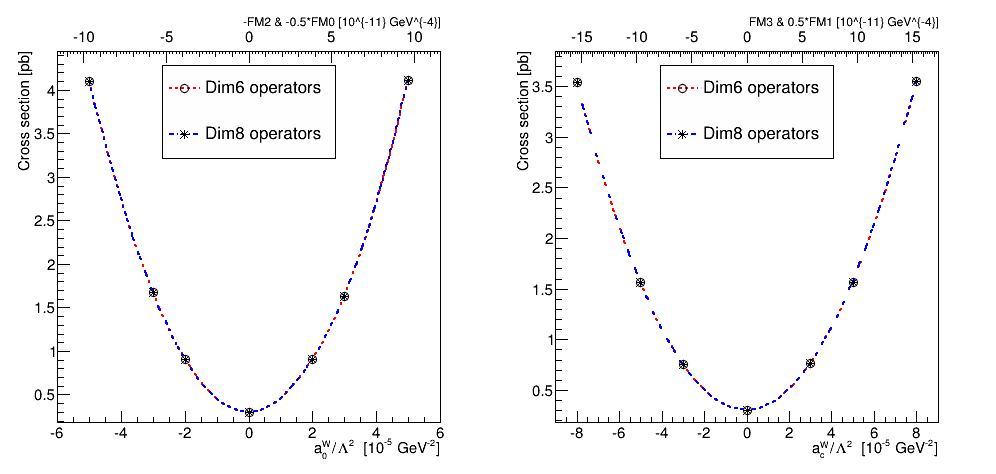
\includegraphics[width=0.8\textwidth]{figs/comp68.png}\\
  \caption{Checking the relations in Eq.s~\ref{dim6to8}}\label{comp}
\end{figure}

where $\dfrac{f_{M,i}}{\Lambda^4}$ are parameters of the linear formalism. We've checked this relation using the $p p \to W^+ W^- \gamma$ process without $W$ boson decay~\ref{comp}.

Moreover, there are more types of aQGC operators appearing in the linear
formalism which have never been tested before. Therefore, as a second
step, we investigate the ${\cal L}_{T,i}$ operators in the linear
formalism~\cite{Eboli:2006wa}, with new lorentz structures, which have
never been tested experimentally.

Therefore, concerning both vertex $WW\gamma \gamma$ and $WWZ\gamma$, the anomalous part of the total lagrangian \eqref{lagrangian} can be rewritten as

\begin{equation}\label{lagrangian}
{\cal L}_{AQGC} = \dfrac{a_0^W}{4 g^2} {\cal W}_{0}^{\gamma} + \dfrac{a_c^W}{4 g^2} {\cal W}_{c}^{\gamma} + \sum_i k_i^{W} {\cal W}_{i}^{Z} + {\cal L}_{T,0} + {\cal L}_{T,1} + {\cal L}_{T,2}
\end{equation}

% dimension 6 operators,  the $WW\gamma \gamma$ vertex, requiring only $U(1)_{EM}$ gauge invariance together with C and P conserved symmetry, arises from two basic Lorentz structures~\cite{Belanger:1999}
%\begin{eqnarray} 
%{\cal W}_{0}^{\gamma} &=& -\dfrac{e^{2}g^{2}}{2\Lambda^{2}}\; F_{\mu \nu} F^{\mu \nu} W^{+\alpha}W^{-}_{\alpha} \rightarrow i\dfrac{e^{2}g^{2}}{\Lambda^{2}}\; 2g_{\alpha \beta} (g_{\mu \nu} k_{1}k_{2}-k_{1\nu}k_{2\mu}) \nonumber \\
%&& \nonumber\\
%{\cal W}_{C}^{\gamma} &=& -\dfrac{e^{2}g^{2}}{4\Lambda^{2}}\; F_{\mu \nu} F^{\mu \alpha} \left( W^{+\nu}W^{-}_{\alpha} + W^{-\nu}W^{+}_{\alpha} \right) \rightarrow i\dfrac{e^{2}g^{2}}{2\Lambda^{2}}\;\left[ (g_{\mu\alpha}g_{\nu\beta}+g_{\nu\alpha}g_{\mu\beta})k_{1}\cdot k_{2} + g_{\mu\nu}(k_{2\beta}k_{1\alpha}+k_{1\beta}k_{2\alpha}) \right . \nonumber \\
%&& \left . \;\;\;\;\;\;\;\;\;\;\;\;\;\;\;\;\;\;\;\;\;\;\;\;\;\;\;\;\;\;\;\;\;\;\;\;\;\;\;\;\;\;\;\;\;\;\;\;\;\;\;\;\;\;\;\;\;\;\;\;\;\;\;\;\;\;\; - k_{2\mu}k_{1\alpha}g_{\nu\beta} - k_{2\beta}k_{1\nu}g_{\mu\alpha} - k_{2\alpha}k_{1\nu}g_{\mu\beta} - k_{2\mu}k_{1\beta}g_{\nu\alpha}   \right]
%\label{em_oper1}
%\end{eqnarray}
%while the $W^{+}W^{-}Z\gamma$ one has a maximum of 5 independent structures
%\begin{eqnarray}
%{\cal W}^{Z}_{0} &=& -\dfrac{e^{2}g^{2}}{\Lambda^{2}}\;F_{\mu\nu}Z^{\mu\nu}W^{+\alpha}W^{-}_{\alpha} \rightarrow i\dfrac{e^{2}g^{2}}{\Lambda^{2}}\; 2g_{\alpha \beta} (g_{\mu \nu} k_{1}k_{2}-k_{1\nu}k_{2\mu}) \nonumber\\
%&& \nonumber\\
%{\cal W}^{Z}_{C} &=& -\dfrac{e^{2}g^{2}}{2\Lambda^{2}}\;F_{\mu\nu}Z^{\mu\alpha} \left( W^{+\nu}W^{-}_{\alpha}+ W^{-\nu}W^{+}_{\alpha} \right) \rightarrow i\dfrac{e^{2}g^{2}}{2\Lambda^{2}}\;\left[ (g_{\mu\alpha}g_{\nu\beta}+g_{\nu\alpha}g_{\mu\beta})k_{1}\cdot k_{2} + g_{\mu\nu}(k_{2\beta}k_{1\alpha}+k_{1\beta}k_{2\alpha}) \right . \nonumber\\
%&& \nonumber\\
%&& \left .  \;\;\;\;\;\;\;\;\;\;\;\;\;\;\;\;\;\;\;\;\;\;\;\;\;\;\;\;\;\;\;\;\;\;\;\;\;\;\;\;\;\;\;\;\;\;\;\;\;\;\;\;\;\;\;\;\;\;\;\;\;\;\;\;\;\;\;- k_{2\mu}k_{1\alpha}g_{\nu\beta} - k_{2\beta}k_{1\nu}g_{\mu\alpha} - k_{2\alpha}k_{1\nu}g_{\mu\beta} - k_{2\mu}k_{1\beta}g_{\nu\alpha}   \right] \nonumber \\
%&&\nonumber\\
%{\cal W}^{Z}_{1} &=& -\dfrac{e^{2}g^{2}g_{Z}}{2\Lambda^{2}}\;F_{\mu\nu} \left( W^{+}_{\mu \nu}W^{-}_{\alpha}Z^{\alpha} + W^{-}_{\mu\nu}W^{+}_{\alpha}Z^{\alpha} \right) \rightarrow i\dfrac{eg^{2}g_{Z}}{\Lambda^{2}}\; \left ( (g_{\mu\alpha }k_{1}\cdot k_{+} - k_{+\mu}k_{1\alpha}  ) g_{\nu\beta}  + (g_{\mu\beta}k_{1}\cdot k_{-} - k_{-\mu} k_{1\beta}) g_{\nu\alpha} \right ) \nonumber\\
%&& \nonumber\\
%{\cal W}^{Z}_{2} &=& -\dfrac{eg^{2}g_{Z}}{2\Lambda^{2}}\;F_{\mu\nu} \left( W^{+}_{\mu \alpha}W^{-}_{\alpha}Z^{\nu} + W^{-}_{\mu\alpha}W^{+\alpha}Z^{\nu} \right) \rightarrow i\dfrac{eg^{2}g_{Z}}{2\Lambda^{2}}\; \left [  (k_{1}\cdot k_{+} + k_{1}\cdot k_{-})g_{\mu\nu}g_{\alpha\beta} - (k_{1\alpha}k_{+\beta} + k_{1\beta}k_{-\alpha})g_{\mu\nu} \right . \nonumber \\
%&& \nonumber \\
%&& \left .  \;\;\;\;\;\;\;\;\;\;\;\;\;\;\;\;\;\;\;\;\;\;\;\;\;\;\;\;\;\;\;\;\;\;\;\;\;\;\;\;\;\;\;\;\;\;\;\;\;\;\;\;\;\;\;\;\;\;\;\;\;\;\;\;\;\;\; - (k_{+\mu}+k_{-\mu})k_{1\nu}g_{\alpha \beta} + (k_{+\beta} g_{\mu\alpha} + k_{-\alpha}g_{\mu\beta} )k_{1\nu}\right] \nonumber \\
%&& \nonumber \\
%{\cal W}^{Z}_{3} &=& -\dfrac{eg^{2}g_{Z}}{2\Lambda^{2}}\;F_{\mu\nu} \left( W^{+}_{\mu \alpha}W^{-}_{\nu}Z^{\alpha} + W^{-}_{\mu\alpha}W^{+}_{\nu}Z^{\alpha} \right) \rightarrow i\dfrac{eg^{2}g_{Z}}{2\Lambda^{2}}\;   ( k_{1}\cdot k_{+} g_{\mu\beta}g_{\nu\alpha} + k_{1}\cdot k_{-} g_{\mu\alpha}g_{\nu\beta} + (k_{+\nu} - k_{-\nu})k_{1\beta} g_{\mu\alpha}  \nonumber \\
%&& \nonumber \\
%&&  \;\;\;\;\;\;\;\;\;\;\;\;\;\;\;\;\;\;\;\;\;\;\;\;\;\;\;\;\;\;\;\;\;\;\;\;\;\;\;\;\;\;\;\;\;\;\;\;\;\;\;\;\;\;\;\;\;\;\;\;\;\;\;\;\;\;\;- (k_{+\nu}-k_{-\nu})k_{1\alpha}g_{\mu\beta} - k_{+\mu}k_{1\beta} g_{\nu\alpha} - k_{-\mu}k_{1\alpha}g_{\nu\beta})
%\label{em_oper2}
%\end{eqnarray}
%where $g=e/s_{W}$ and $g_{Z}=e/c_{W}s_{W}$.

%In order to embed the set of operators \eqref{em_oper1} and \eqref{em_oper2}  in manifestly $SU(2)\times U(1)$ gauge invariant and $SU(2)_{C}$ symmetric operators (as well as C and P conserving),  one uses the chiral Lagrangian approach which assumes no Higgs in the spectrum (a Higgsless scenario).

%In this scenario, concerning the purely bosonic sector, the $SU(2)$ kinetic term that originates the standard tree-level gauge self-coulplings is
%\begin{equation}
%{\cal L}_{Gauge} = -\dfrac{1}{2} \left[ \mbox{Tr}(\mathbf{W}_{\mu\nu}\mathbf{W^{\mu\nu}} +\mbox{Tr}(\mathbf{B}_{\mu\nu}\mathbf{B}^{\mu\nu} )  \right]
%\end{equation}
% where the $SU(2)$ gauge fields are $\mathbf{W}_{\mu}=W_{\mu}^{i}\tau^{i}$ and the hypercharge is denoted by $\mathbf{B}_{\mu}=\tau_{3}B_{\mu}$. The normalization for the Pauli matrices is $\mbox{Tr}(\tau^{i}\tau^{j})=2\delta^{ij}$. The field strength is  defined as
%\begin{equation}
%\mathbf{W}_{\mu\nu} = \dfrac{1}{2}\left( \partial_{\mu}\mathbf{W}_{\nu} - \partial_{\nu}\mathbf{W}_{\mu} + \dfrac{i}{2}\;g\;[\mathbf{W}_{\mu},\mathbf{W}_{\nu}]   \right) = \dfrac{\tau^{i}}{2} \left ( \partial_{\mu}W_{\nu} - \partial_{\nu}W_{\mu} -\;g\;\epsilon^{ijk} W_{\mu}^{j} W_{\nu}^{k}  \right )
%\end{equation} 

%Choosing a matrix field $\Sigma$ to acommodate the Goldstone bosons $w^{i}$ , with $i=1,2,3$, we have
%\begin{equation}
%\Sigma = \exp{i(\frac{w^{i}\tau^{i}}{v})}\;\;\mbox{with covariant derivative as}\;\; D_{\mu}\Sigma = \partial_{\mu}\Sigma+ \frac{i}{2} (g\mathbf{W}_{\mu}\Sigma - g'\;\mathbf{B}_{\mu}\Sigma \tau_{3}  )
%\end{equation}
%where $v=246$~GeV , $g=e/s_{W}$ and $g'=e/c_{W}$.


%Defining the matrix field $\mathbf{V}_{\mu}=(D_{\mu}\Sigma)\Sigma^{\dagger}$, we note that in the unitary gauge $\mathbf{V}_{\mu}$ corresponds to the triplet of the massive gauge bosons $W^{\pm},Z$. Indeed, in the unitary gauge $\Sigma=\mathbf{1}$ and then $\mathbf{V}_{\mu}=D_{\mu}\mathbf{1}=i (g\mathbf{W}_{\mu}-g'\mathbf{B}_{\mu})$ where $\mathbf{W}_{\mu}= \dfrac{\vec{W}_{\mu}\cdot \vec{\tau}}{2}$ and  $\mathbf{B}_{\mu}= \dfrac{B_{\mu}\cdot \tau_{3}}{2}$.

%The NLO in the chiral Lagrangian approach (dimension 4) gives genuine quartic couplings involving massive vector bosons $WWWW$, $WWZZ$, $ZZZZ$ which are out of the scope of our analysis. No photonic operators arises in this perturbation order expansion.

%Photonic operators only appear at NNLO (dimension 6).  Although these NNLO operators also involve quartic couplings between massive gauge bosons, for the sake of simplicity we restrict our list only for the photonic part we are interested in.
%\begin{eqnarray}
%&&\dfrac{k_{0,C}^{w}}{\Lambda^{2}}\;g^{2}\;\mbox{Tr}(\mathbf{W}_{\mu\nu}\mathbf{W}^{\mu\nu})\mbox{Tr}(\mathbf{V}^{\alpha}\mathbf{V}_{\alpha}) + \dfrac{k_{0,C}^{b}}{\Lambda^{2}}\;g^{\prime 2}\;\mbox{Tr}(\mathbf{B}_{\mu\nu}\mathbf{B}^{\mu\nu})\mbox{Tr}(\mathbf{V}^{\alpha}\mathbf{V}_{\alpha}) + \dfrac{k_{0,C}^{m}}{\Lambda^{2}}\;gg^{\prime}\;\mbox{Tr}(\mathbf{W}_{\mu\nu}\mathbf{B}^{\mu\nu})\mbox{Tr}(\mathbf{V}^{\alpha}\mathbf{V}_{\alpha}) \nonumber \\
%&+&\dfrac{k_{1}^{w}}{\Lambda^{2}}\;g^{2}\;\mbox{Tr}(\mathbf{W}_{\mu\nu}\mathbf{V}^{\alpha})\mbox{Tr}(\mathbf{W}_{\mu\nu}\mathbf{V}_{\alpha}) + \dfrac{k_{2}^{w}}{\Lambda^{2}}\;g^{2}\;\mbox{Tr}(\mathbf{W}_{\mu\nu}\mathbf{V}^{\nu})\mbox{Tr}(\mathbf{W}_{\mu\alpha}\mathbf{V}_{\alpha} + \dfrac{k_{3}^{w}}{\Lambda^{2}}\;g^{2}\;\mbox{Tr}(\mathbf{W}_{\mu\nu}\mathbf{V}_{\alpha})\mbox{Tr}(\mathbf{W}^{\mu\alpha}\mathbf{V}^{\nu})\nonumber \\
%&+&\dfrac{k_{1}^{m}}{\Lambda^{2}}\;gg^{\prime}\;\mbox{Tr}(\mathbf{W}_{\mu\nu}\mathbf{V}^{\alpha})\mbox{Tr}(\mathbf{B}_{\mu\nu}\mathbf{V}_{\alpha}) +\dfrac{k_{2}^{m}}{\Lambda^{2}}\;gg^{\prime}\;\mbox{Tr}(\mathbf{W}_{\mu\nu}\mathbf{V}^{\nu})\mbox{Tr}(\mathbf{B}_{\mu\alpha}\mathbf{V}_{\alpha}) + \dfrac{k_{3}^{m}}{\Lambda^{2}}\;gg^{\prime}\;\mbox{Tr}(\mathbf{W}_{\mu\nu}\mathbf{V}^{\alpha})\mbox{Tr}(\mathbf{B}_{\mu\alpha}\mathbf{V}_{\nu}) \nonumber \\
%\label{dim6}
%\end{eqnarray}

%In this way, for the photonic vertices $WW\gamma \gamma$ and $WWZ\gamma$, looking only at features of the non-linearly built dimension 6 operators of the set \eqref{dim6}, we can construct the lagrangians ${\cal L}_{0}^{6}$ and ${\cal L}_{C}^{6}$ as follows

%\begin{equation}
% {\cal L}_{\{0,C\}}^{6}= (k_{0,C}^{w}+  k_{0,C}^{b} + k_{0,C}^{m}) {\cal W}_{0}^{\gamma}  + (\dfrac{c_{W}}{s_{W}} k_{0,C}^{w}- \dfrac{s_{W}}{c_{W}} k_{0,C}^{b} +c_{ZW}k_{0,C}^{m}) {\cal W}_{0}^{Z}
%\end{equation}
%where
%\[
%c_{ZW}\equiv \mbox{cotg}{(2\theta_{W})} = \dfrac{c^{2}_{W}- s^{2}_{W}}{2c_{W}s_{W}}.
%\]

%Moreover, the vertex $WWZ\gamma$ has other specific contributing terms, we may name as ${\cal L}_{Z}^{6}$, like 
%\begin{equation}
% {\cal L}_{Z}^{6}= (k_{1}^{w}+ k_{1}^{m}){\cal W}_{1}^{Z} +(k_{2}^{w} + k_{2}^{m}){\cal W}_{2}^{Z} + (k_{3}^{w} + k_{3}^{m}){\cal W}_{3}^{Z}
%\label{LZ}
%\end{equation}

%Therefore, while for $WW\gamma \gamma$ we can compute "only" its corresponding part at ${\cal L}_{0}$ and ${\cal L}_{C}$,  for the $WWZ\gamma$ vertex we have to consider, beyond its corresponding part at  ${\cal L}_{0}$ and ${\cal L}_{C}$, also the ${\cal L}_{Z}$ contribution.

%The LEP collaboration has adopted the set of operators \eqref{em_oper1} to infer constraints on their $a_{0}$ and $a_{C}$ parameters. In order to make a comparison with these previous results,  we may relate parameters conveniently. This goal in mind, by assuming $k_{1,2,3}^{w,m}=0$ (since they do not contribute to $WW\gamma \gamma$) and the constraints
%\begin{equation}
%k_{0,C}^{w} = k_{0,C}^{\gamma} s^{2}_{W} \;\;\;\;\;, \;\;\;\;\; k_{0,C}^{b} = k_{0,C}^{\gamma} c^{2}_{W},  
%\end{equation}
%we obtain only two independent parameters controlling $WW\gamma\gamma$ vertex, making the following contact with the operators analyzed by LEP
%\begin{equation}
%a_{0,C}=4g^{2}(k_{0,C}^{b}+k_{0,C}^{w}+k_{0,C}^{m}) = 4g^{2}k_{0,C}^{\gamma}.
%\end{equation}

% In general, using a manifestly gauge invariant and $SU(2)_{C}$ symmetric approach, the operators which contribute to $WW\gamma\gamma$, $k_{0,C}^{w,b,m}$ do in general induce a $WWZ\gamma$ vertex as well. Therefore, with $k_{1,2,3}^{w,m}=0$ the general condition for the vanishing of $WWZ\gamma$ is
%\begin{equation}
%2k_{0,C}^{w}+k_{0,C}^{m}=2\sin^{2}{\theta_{W}}\;(k_{0,C}^{b}+k_{0,C}^{w}+k_{0,C}^{m})
%\end{equation}
%with
%\begin{equation}
%k_{0,C}^{b}+k_{0,C}^{w}+k_{0,C}^{m} \neq 0
%\end{equation}
%of course not making the $VV\gamma \gamma$ vanish.

%On the other hand one can also arrange the operators such that $SU(2)_{C}$ $WW\gamma\gamma$ couplings vanish so that effectively $a_{0,C}=0$ but not the quartic $WWZ\gamma$ one. For instance, with all $k_{1,2,3}=0$ , this can achieved by having $k_{0,C}^{b}=-k_{0,C}^{w}$.

%Up to now we have adopted an effective lagrangian approach which does not assume a Higgs-like field on the spectrum of the theory. Nevertheless, any operator can be made gauge invariant with the Higgs presence, only changing the hierarchy in the couplings changes, realizing the symmetry linearly. 

%Assuming a scenario where the low energy spectrum contains a light Higgs boson, we
%can choose a linear realization of the symmetry breaking in the form of
%the usual scalar doublet field $\Phi$,
%\[
%\Phi = \dfrac{1}{\sqrt{2}}\begin{pmatrix} 0 & v+ H \end{pmatrix}^{T},
%\]
%where $v=246$~GeV.

%The basic blocks for constructing the operators which can modify the 
%quartic gauge boson vertices are the covariant derivative of the Higgs
%field $D_{\mu}\Phi$,  the $SU(2)_{L}$ field strength 
%$\hat{W}_{\mu \nu}$, and the $U(1)_{Y}$ field strength 
%$\hat{B}_{\mu \nu}$ listed bellow.

%\begin{eqnarray}
%\Phi &\mbox{, transforming as} & \Phi^{\prime}=U\Phi \\
%D_{\mu}\Phi &\mbox{, transforming as} & D^{\prime}_{\mu}\Phi^{\prime}=UD_{\mu}\Phi \\
%\hat{W}_{\mu \nu}\equiv i\frac{g}{2}\sum_{j}W^{j}_{\mu \nu}\sigma^{j} &\mbox{, transforming as} & \hat{W}^{\prime}_{\mu \nu}= U\hat{W}_{\mu\nu}U^{\dagger} \\
%\hat{B}_{\mu \nu}=i\frac{g^{\prime}}{2}B_{\mu \nu} &\mbox{, transforming as} & B^{\prime}_{\mu \nu}=B_{\mu \nu}
%\label{linear_blocks}
%\end{eqnarray}

%where the covariant derivative is given by 
%\[
%D_{\mu} = \partial_{\mu}+i\frac{g}{2}W^{j}_{\mu}\sigma^{j}+i\frac{g^{\prime}}{2}B_{\mu}, 
%\]

%\[
%\left[ D_{\mu}, D_{\nu} \right]=\hat{W}_{\mu \nu}+\hat{B}_{\mu \nu},
%\]

%and

%\begin{eqnarray}
%W^{j}_{\mu \nu}&=&\partial _{\mu}W^{j}_{\nu}-\partial_{\nu}W^{j}_{\mu}+g\epsilon_{jkm}W_{\mu}^{k}W_{\nu}^{m},\\
%B_{\mu \nu}&=& \partial_{\mu}B_{\nu}-\partial_{\nu}B_{\mu}.
%\end{eqnarray}

%In this context, the lowest dimension operator that leads to pure 
%quartic interactions (not exhibiting two or three real gauge boson 
%vertices) is dimension 8. Many CP conserving effective dim-8 operators 
%were already listed elsewhere~\cite{Eboli:2006wa}. Here we have 
%manipulated operators showing only $WW\gamma\gamma$ and $WWZ\gamma$ 
%vertices.

%From the linear realized symmetry scenario emerges dimension 8 operators which shows a trivial equivalence with the already built dimension 6 ones, ${\cal L}_{\{0,C\}}^{6}$,  as
%\begin{eqnarray}
%{\cal L}_{0}^{8} &=& g^{\prime 2}\; \dfrac{Q_{0}^{b}}{\Lambda^{4}} (D_{\beta}\Phi)(D^{\beta}\Phi)^{\dagger} B_{\mu\nu}B^{\mu\nu} + g^{2}\; \dfrac{Q_{0}^{w}}{\Lambda^{4}} (D_{\beta}\Phi)(D^{\beta}\Phi)^{\dagger} W^{i}_{\mu\nu}W^{i\mu\nu} + gg^{\prime}\; \dfrac{Q_{0}^{m}}{\Lambda^{4}} (D_{\beta}\Phi)(D^{\beta}\Phi)^{\dagger} W^{3}_{\mu\nu}B^{\mu\nu}  \nonumber\\
%&& \nonumber\\
%&& \nonumber\\
%{\cal L}_{C}^{8} &=& g^{\prime 2}\; \dfrac{Q_{C}^{b}}{2\Lambda^{4}} (D^{\alpha}\Phi)(D_{\beta}\Phi)^{\dagger} B_{\mu\alpha}B^{\mu\beta} + g^{2}\; \dfrac{Q_{C}^{w}}{2\Lambda^{4}} (D^{\alpha}\Phi)(D_{\beta}\Phi)^{\dagger} W^{i}_{\mu\alpha}W^{i\mu\beta} + gg^{\prime}\; \dfrac{Q_{C}^{m}}{2\Lambda^{4}} (D^{\alpha}\Phi)(D_{\beta}\Phi)^{\dagger} W^{3}_{\mu\alpha}B^{\mu\beta}\nonumber \\
%\label{dim8_belanger}
%\end{eqnarray}

%where one can make a trivial correspondence both scenario between parameters as 
%\begin{equation}
%\dfrac{Q^{b,w,m}_{0,C}}{\Lambda^{2}} =-\dfrac{1}{2}\dfrac{g^{2}}{M_{W}^{2}}\; k_{0,C}^{b,w,m}.
%\label{relation}
%\end{equation}

%To measure the deviation from the SM lagrangian, we are interested on the following effective lagrangian based upon the operators listed so far

%\begin{equation}
%{\cal L}_{Total}= {\cal L}_{SM} + {\cal L}_{ANOM}
%\label{lagrangian}
%\end{equation}

%which contributes to the squared matriz element as
%\begin{equation}
%|{\cal M}_{Total}|^{2}= |{\cal M}_{SM}+{\cal M}_{AQGC} |^{2} =  |{\cal M}_{SM}|^{2}+|{\cal M}_{AQGC} |^{2} + ({\cal M}^{*}_{SM}{\cal M}_{AQGC} + {\cal M}_{SM}{\cal M}^{*}_{AQGC})
%\end{equation}
%, $M_{W}=gv/2$, $M_{Z}=g_{Z}v/2$ with
%Since the squared matrix element is proportional to the cross section then we may parameterize the total cross section for the process $pp\to l\nu_{ll}jj\gamma$ as a quadratic function
%\begin{equation}
%\sigma_{total} \equiv \sigma_{SM} + \beta\sigma_{INT} +\beta^{2}\sigma_{AQGC}
%\end{equation}
%where $\sigma_{SM}$,  $\sigma_{INT}$, $\sigma_{AQGC}$ are  Standard Model cross section, interference between the SM and the anomalous contributions and the pure anomalous cross section, respectively.

%%Therefore, concerning both vertex $WW\gamma \gamma$ and $WWZ\gamma$, the anomalous part of the total lagrangian \eqref{lagrangian} may be rewritten as

%\begin{equation}
%{\cal L}_{AQGC}= {\cal L}_{0}^{6} + {\cal L}_{C}^{6} +{\cal L}_{Z}^{6} + {\cal L}_{T0,5} + {\cal L}_{T1,6} + {\cal L}_{2,7}
%\end{equation}
%where ${\cal L}_{Z}^{6}={\cal L}_{1}+{\cal L}_{2}+{\cal L}_{3}$ is the expression  \eqref{LZ} and the additional operators named ${\cal L}_{T0,5}$, ${\cal L}_{T1,6}$ and ${\cal L}_{2,7}$, listed below in the set of Eqs. \eqref{lt_operators}, are linearly realized dimension 8 effective operators which were not yet probed before.

%In the following we listed other dimension 8 operators related to our analysis~~\cite{Eboli:2006wa}.

%\begin{itemize}
%\item Structure compatible with ${\cal L}_{0}^{8}$
%\begin{eqnarray}
%{\cal L}_{M,\{2+0+4\}} &=& \dfrac{f_{M2}}{\Lambda^{4}}\;\mbox{Tr}\left[ \mathbf{B}_{\mu\nu} \mathbf{B}^{\mu\nu}\right] \times \left[  (D_{\beta}\Phi)^{\dagger} D^{\beta}\Phi \right] + \dfrac{f_{M0}}{\Lambda^{4}}\;\mbox{Tr}\left[ \mathbf{W}_{\mu\nu} \mathbf{W}^{\mu\nu}\right] \times \left[  (D_{\beta}\Phi)^{\dagger} D^{\beta}\Phi \right] \nonumber \\
%&& \nonumber \\
%&&+ \dfrac{f_{M4}}{\Lambda^{4}}\;\left[  (D_{\beta}\Phi)^{\dagger} \mathbf{W}^{\beta\nu}  D^{\mu}\Phi \right] \times \mathbf{B}^{\beta\nu} \nonumber \\
%&& \nonumber\\
%&\rightarrow&  i\; g^{2}m_{W}^{2}s^{2}_{W} \; \dfrac{(f_{M2}+2f_{M0}+f_{M4})}{\Lambda^{4}}\; g^{\mu\nu} (g^{a_{1}a_{2}}p_{\lambda_{1}}p_{\lambda_{2}} - p_{\lambda_{2}}^{a_{1}} p_{\lambda_{1}}^{a_{2}})
%\label{dim8_a}
%\end{eqnarray}

%\item Structure compatible with ${\cal L}_{C}^{8}$
%\begin{eqnarray}
%{\cal L}_{M,\{3+1+5\}} &=& \dfrac{f_{M3}}{\Lambda^{4}}\;\mbox{Tr}\left[ \mathbf{B}_{\mu\nu} \mathbf{B}^{\nu\beta}\right] \times \left[  (D_{\beta}\Phi)^{\dagger} D^{\mu}\Phi \right] + \dfrac{f_{M1}}{\Lambda^{4}}\;\mbox{Tr}\left[ \mathbf{W}_{\mu\nu} \mathbf{W}^{\nu\beta}\right] \times \left[  (D_{\beta}\Phi)^{\dagger} D^{\mu}\Phi \right] \nonumber \\
%&& \nonumber \\
%&& + \dfrac{f_{M5}}{\Lambda^{4}}\;\left[  (D_{\mu}\Phi)^{\dagger} \mathbf{W}^{\beta\nu}  D^{\nu}\Phi \right] \times \mathbf{B}^{\beta\nu} \nonumber \\
%&& \nonumber \\
%&\rightarrow& i \; g^{2}m_{W}^{2}s^{2}_{W} \; \dfrac{((1/4)f_{M3}+(1/2)f_{M1}+(1/4)f_{M5})}{\Lambda^{4}}\; \left (   - p_{\lambda_{2}}^{a_{1}} ( p^{\nu}_{\lambda_{1}}g^{a_{2}\mu} + p_{\lambda_{1}}^{\mu}g^{a_{2}\nu})  \right . \nonumber \\
%&& \nonumber \\
%&& \left .-  p_{\lambda_{1}}^{a_{2}} ( p^{\nu}_{\lambda_{2}}g^{a_{1}\mu} + p_{\lambda_{2}}^{\mu}g^{a_{1}\nu})+ g^{a_{1}a_{2}} ( p^{\mu}_{\lambda_{1}}p_{\lambda_{2}}^{\nu} + p_{\lambda_{1}}^{\nu}  p^{\mu}_{\lambda_{2}}) + p_{\lambda_{1}}\cdot p_{\lambda_{2}} ( g^{a_{1}\mu}g^{a_{2}\nu} +g^{a_{1}\nu}g^{a_{2}\mu} ) \right )\nonumber \\
%\label{dim8_b}
%\end{eqnarray}

%\item Not directly related with dimension 6 ones.
%\begin{eqnarray}
%{\cal L}_{T,\{0+5\}} &=&\dfrac{f_{T0}}{\Lambda^{4}}\;\mbox{Tr}\left[ \mathbf{W}_{\mu\nu} \mathbf{W}^{\mu\nu}\right] \times \mbox{Tr}\left[ \mathbf{W}_{\alpha\beta} \mathbf{W}^{\alpha\beta}\right] +  \dfrac{f_{T5}}{\Lambda^{4}}\;\mbox{Tr}\left[ \mathbf{W}_{\mu\nu} \mathbf{W}^{\mu\nu}\right] \times \mathbf{B}_{\alpha\beta} \mathbf{B}^{\alpha\beta} \nonumber \\
%&\rightarrow& i \;s^{2}_{W}g^{4}\;\dfrac{(8f_{T0}+2f_{T5})}{\Lambda^{4}}\; [(p_{\gamma_{2}}^{a_{1}}  p_{\gamma_{1}}^{a_{2}} - g^{a_{1}a_{2}} p_{\gamma_{1}}\cdot p_{\gamma_{2}}) (p_{-}^{\mu}p_{+}^{\nu}-g^{\nu\mu}p_{-}\cdot p_{+})] \nonumber \\
%&& \nonumber \\
%&& \nonumber \\
%{\cal L}_{T,\{1+6\}} &=& \dfrac{f_{T1}}{\Lambda^{4}}\;\mbox{Tr}\left[ \mathbf{W}_{\alpha\nu} \mathbf{W}^{\mu\beta}\right] \times \mbox{Tr}\left[ \mathbf{W}_{\mu\beta} \mathbf{W}^{\alpha\nu}\right] +  \dfrac{f_{T6}}{\Lambda^{4}}\;\mbox{Tr}\left[ \mathbf{W}_{\alpha\nu} \mathbf{W}^{\mu\beta}\right] \times \mathbf{B}_{\mu\beta} \mathbf{B}^{\alpha\nu} \nonumber\\
%&& \nonumber \\
%&\rightarrow& i\;s^{2}_{W}g^{4} \;\dfrac{(4f_{T1}+f_{T6})}{\Lambda^{4}}\; \left ( (p_{+}^{a_{1}}p_{\gamma_{1}}^{\mu} - g^{a_{1}\mu}p_{\gamma_{1}}\cdot p_{+} ) (p_{-}^{a_{2}}p_{\gamma_{2}}^{\nu} - g^{a_{2}\nu}p_{\gamma_{2}}\cdot p_{-} ) \right . \nonumber \\
%&& \nonumber \\
%&& + \left . (p_{-}^{a_{1}}p_{\gamma_{1}}^{\nu} - g^{a_{1}\nu}p_{\gamma_{1}}\cdot p_{-}) + (p_{+}^{a_{2}}p_{\gamma_{2}}^{\mu} - g^{a_{2}\mu}p_{\gamma_{2}}\cdot p_{+} ) \right) \nonumber \\
%&& \nonumber \\ 
%&& \nonumber \\
%{\cal L}_{T,\{2+7\}} &=& \dfrac{f_{T2}}{\Lambda^{4}}\;\mbox{Tr}\left[ \mathbf{W}_{\alpha\mu} \mathbf{W}^{\mu\beta}\right] \times \mbox{Tr}\left[ \mathbf{W}_{\beta\nu} \mathbf{W}^{\nu\alpha}\right] + \dfrac{f_{T7}}{\Lambda^{4}}\;\mbox{Tr}\left[ \mathbf{W}_{\alpha\mu} \mathbf{W}^{\mu\beta}\right] \times \mathbf{B}_{\beta\nu} \mathbf{B}^{\nu\alpha} \nonumber \\
%&& \nonumber \\
%&\rightarrow& i\;s^{2}_{W}g^{4} \;\dfrac{(f_{T2}+(1/4)f_{T7})}{\Lambda^{4}}\; \left \{ g^{a_{1}a_{2}}g^{\mu\nu} (p_{\lambda_{1}}\cdot p_{+}\;p_{\lambda_{2}} \cdot p_{-} + p_{\lambda_{1}}\cdot p_{-}\;p_{\lambda_{2}}\cdot p_{+}) \right .\nonumber \\
%&& \nonumber \\
%&& g^{\mu\nu} \left[ - p^{a_{1}}_{\lambda_{2}} ( p_{+}^{a_{2}}\;p_{\lambda_{1}} \cdot p_{-} + p^{a_{2}}_{-} p_{\lambda_{1}}\cdot p_{+} ) + p_{+}^{a_{1}} ( p_{-}^{a_{2}}\; p_{\lambda_{1}} \cdot p_{\lambda_{2}}  -  p_{\lambda_{1}}^{a_{2}}\; p_{\lambda_{2}}\cdot p_{-}  ) \right .\nonumber \\
%&& \nonumber \\
%&& \left .+p^{a_{1}}_{-} ( p_{+}^{a_{2}}\; p_{\lambda_{1}}\cdot p_{\lambda_{2}} -  p_{\lambda_{1}}^{a_{2}}\;p_{\lambda_{2}}\cdot p_{+}) \right] \nonumber \\
%&& \nonumber \\
%&& g^{a_{1}\mu}g^{a_{2}\nu} p_{\lambda_{1}}\cdot p_{\lambda_{2}} \; p_{-} \cdot p_{+} + 
%g^{a_{1}\nu}g^{a_{2}\mu} p_{\lambda_{1}}\cdot p_{\lambda_{2}}\; p_{-}\cdot p_{+} \nonumber\\
%&& \nonumber \\
%&&  - g^{a_{1}a_{2}} \left[  p^{\nu}_{+} ( p_{\lambda_{2}}^{\mu}\;p_{\lambda_{1}} \cdot p_{-} + p^{\mu}_{\lambda_{1}}\; p_{\lambda_{2}}\cdot p_{-} ) + p_{-}^{\mu} ( p_{\lambda_{2}}^{\nu}\; p_{\lambda_{1}} \cdot p_{+}  +  p_{\lambda_{1}}^{\nu}\; p_{\lambda_{2}}\cdot p_{+}  ) \right .\nonumber \\
%&& \nonumber \\
%&& \left. -p_{-}\cdot p_{+} \; ( p_{\lambda_{1}}^{\mu}p_{\lambda_{2}}^{\nu} + p_{\lambda_{1}}^{\nu} + p_{\lambda_{2}}^{\mu}) \right] \nonumber \\
%&& \nonumber \\
%&& - g^{a_{2}\mu} ( p_{-}^{a_{1}}p_{+}^{\nu}\;p_{\lambda_{1}}\cdot p_{\lambda_{2}} + p_{\lambda_{2}}^{a_{1}} ( p_{\lambda_{1}}^{\nu}p_{-}\cdot p_{+} - p_{+}^{\nu} p_{\lambda_{1}} \cdot p_{-} ) ) \nonumber \\
%&& \nonumber \\
%&& -  g^{a_{1}\mu} ( p_{-}^{a_{2}}p_{+}^{\nu}\;p_{\lambda_{1}}\cdot p_{\lambda_{2}} + p_{\lambda_{1}}^{a_{2}} ( p_{\lambda_{2}}^{\nu}p_{-}\cdot p_{+} - p_{+}^{\nu} p_{\lambda_{2}} \cdot p_{-} ) ) \nonumber \\
%&& \nonumber \\
%&& - g^{a_{2}\nu} ( p_{+}^{a_{1}}p_{-}^{\mu}\;p_{\lambda_{1}}\cdot p_{\lambda_{2}} + p_{\lambda_{2}}^{a_{1}} ( p_{\lambda_{1}}^{\mu}p_{-}\cdot p_{+} - p_{-}^{\nu} p_{\lambda_{1}} \cdot p_{+} ) ) \nonumber \\
%&& \nonumber \\
%&& - g^{a_{1}\nu} ( p_{+}^{a_{2}}p_{-}^{\mu}\;p_{\lambda_{1}}\cdot p_{\lambda_{2}} + p_{\lambda_{1}}^{a_{2}} ( p_{\lambda_{2}}^{\mu}p_{-}\cdot p_{+} - p_{-}^{\mu} p_{\lambda_{2}} \cdot p_{+} ) ) \nonumber \\
%&& \nonumber \\
%&& + \left . p_{\lambda_{2}}^{a_{1}} p_{-}^{a_{2}}  p_{\lambda_{1}}^{\mu} p_{+}^{\nu} + p_{-}^{a_{1}} p_{\lambda_{1}}^{a_{2}}  p_{\lambda_{2}}^{\mu} p_{+}^{\nu} + p_{\lambda_{2}}^{a_{1}} p_{+}^{a_{2}}  p_{\lambda_{1}}^{\nu} p_{-}^{\nu} + p_{+}^{a_{1}} p_{\lambda_{1}}^{a_{2}}  p_{\lambda_{2}}^{\nu} p_{-}^{\mu}   \right \}
%\label{lt_operators}
%\end{eqnarray}

%\end{itemize}

%\begin{figure}[!htb]
%\centering
%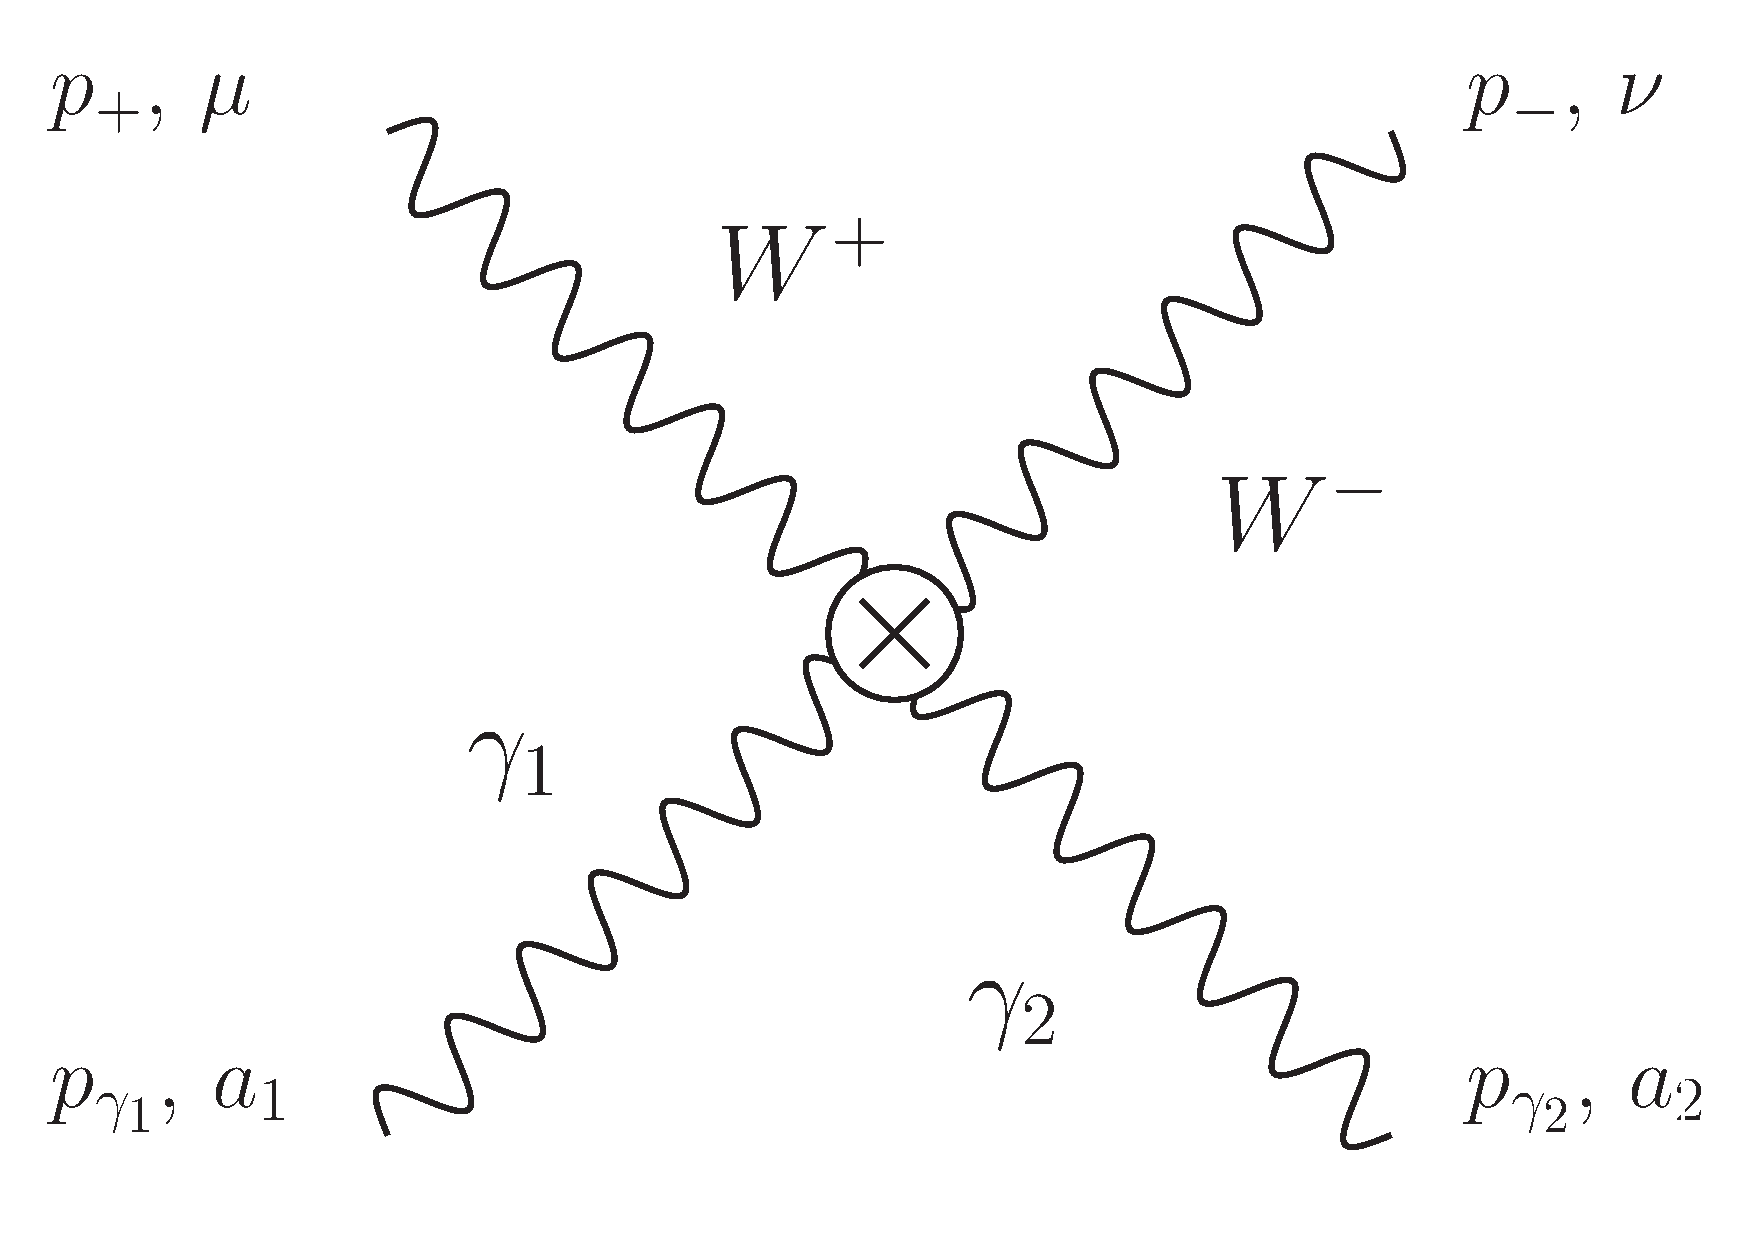
\includegraphics[scale=0.25]{WWAA}
%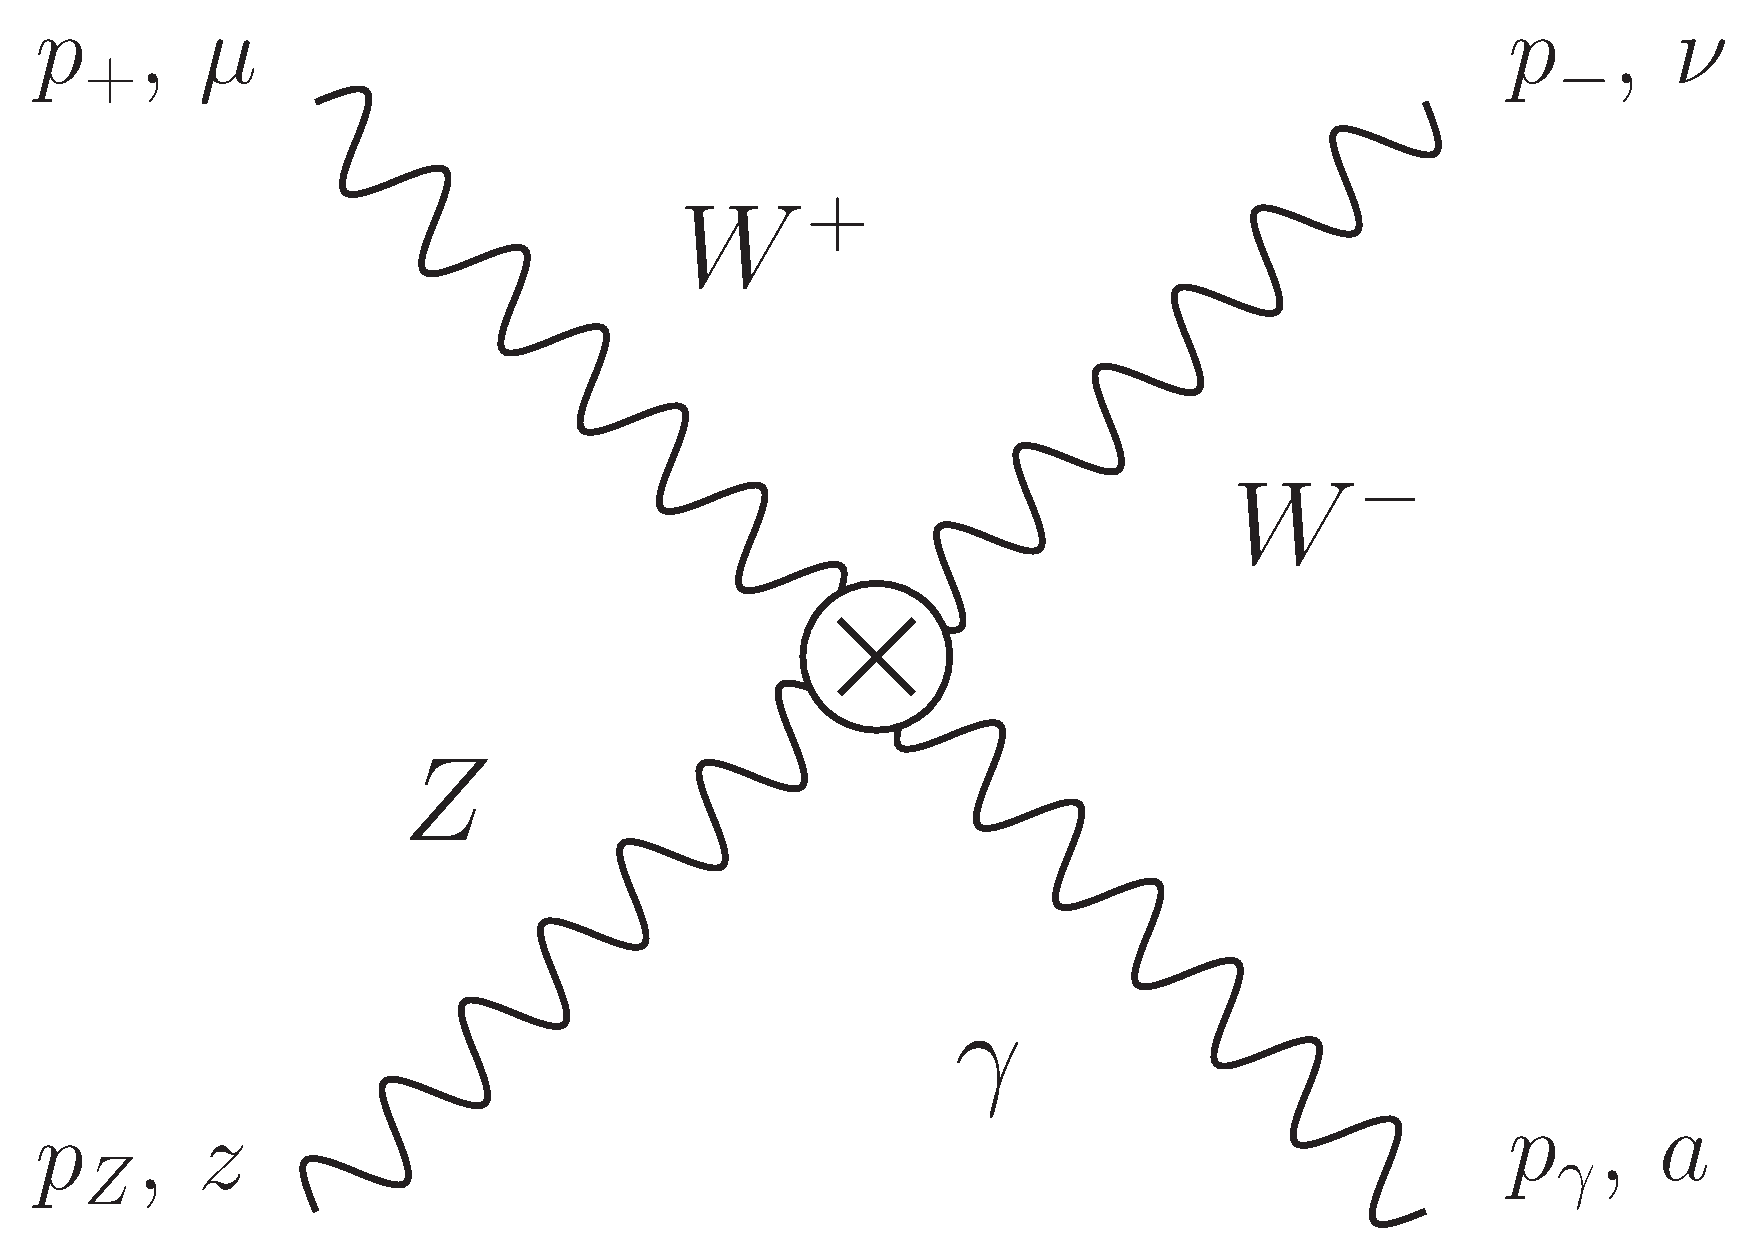
\includegraphics[scale=0.25]{WWZA}
%\end{figure}

%For the vertices $WW\gamma \gamma$ and $WWZ\gamma$, looking at linearly builded dimension 8 operators Eqs. \eqref{dim8_a} and \eqref{dim8_b} and comparing them with Eqs.\eqref{dim8_belanger} together with the relation Eq.\eqref{relation}
%we have
%\begin{eqnarray}
%\dfrac{f_{M2}}{\Lambda^{4}} &=& \dfrac{g^{\prime 2}}{2M_{W}^{4}s^{2}_{W}}\;\dfrac{k_{0}^{b}}{\Lambda^{2}} \nonumber \\
%&& \nonumber\\
%\dfrac{f_{M0}}{\Lambda^{4}} &=& \dfrac{g^{2}}{4M_{W}^{4} s^{2}_{W} }\;\dfrac{k_{0}^{w}}{\Lambda^{2}} \nonumber \\
%&& \nonumber \\
%\dfrac{f_{M4}}{\Lambda^{4}} &=& \dfrac{g\;g^{\prime}}{2M_{W}^{4}s^{2}_{W}}\;\dfrac{k_{0}^{m}}{\Lambda^{2}} \nonumber \\
%&& \nonumber \\
%\dfrac{f_{M3}}{\Lambda^{4}} &=& \dfrac{g^{\prime 2}}{M_{W}^{4}s^{2}_{W}}\;\dfrac{k_{C}^{b}}{\Lambda^{2}}\nonumber \\
%&& \nonumber \\
%\dfrac{f_{M1}}{\Lambda^{4}} &=& \dfrac{g^{2}}{2M_{W}^{4}s^{2}_{W}}\;\dfrac{k_{C}^{w}}{\Lambda^{2}} \nonumber \\
%&& \nonumber \\
%\dfrac{f_{M5}}{\Lambda^{4}} &=& \dfrac{g\;g^{\prime}}{M_{W}^{4}s^{2}_{W}}\;\dfrac{k_{C}^{m}}{\Lambda^{2}}
%\end{eqnarray}

%where $g=e/s_{W}$ and $g^{\prime}=e/c_{W}$.


%In this section, we introduce models we used for our analysis. Instead 
%of studying specific new physics, one can construct an effective 
%Lagrangian in a model-independent way for the anomalous quartic 
%couplings. To build up a resonable model, as a first step, we study the
%lowest possible order operators, which reads 
%6~\cite{500GeVNLC,Belanger:1999}, just as the OPAL group did for LEP 
%analysis ~\cite{wwaLEP:1999,wwaLEP:2004}. In this model, we assume the 
%operators keep $SU(2)_{L} \otimes U(1)_{Y}$ symmetry and $\cal{C}$, 
%$\cal{P}$ independently. In order to fulfill the stringent experimental
%constraint on the $\rho$ parameter, we further require the $SU(2)_C$ 
%custodial symmetry. As for \wwa production, the following structures 
%are included for \wwaa and \wwza 
%interactions~\cite{Belanger:1999,Bosonic:2004PRD}: 

%\begin{center}
%\begin{eqnarray}
% {\cal W}_{0}^{\gamma} = - \frac{e^2 g^2}{2} F_{\mu \nu} F^{\mu \nu} W^{+\alpha} W^{-}_{\alpha} , \\ 

% {\cal W}_{c}^{\gamma} = - \frac{e^2}{16} F_{\mu \nu} F^{\mu \alpha} ( W^{+ \nu} W^{-}_{\alpha} + W^{- \nu} W^{+}_{\alpha} ) , \\

% {\cal W}_{0}^{Z} = - e^2 g^2 F_{\mu \nu} Z^{\mu \nu} W^{+ \alpha} W^{-}_{\alpha} , \\

% {\cal W}_{c}^{Z} = - \frac{e^2 g^2}{2} F_{\mu \nu} Z^{\mu \alpha} ( W^{+ \nu} W^{-}_{\alpha} + W^{- \nu} W^{+}_{\alpha} ) , \\

% {\cal W}_{1}^{Z} = - \frac{e^2 g^2}{2 c_w s_w} F^{\mu \nu} ( W_{\mu \nu}^{+} W_{\alpha}^{-} Z^{\alpha} + W_{\mu \nu}^{-} W_{\alpha}^{+} Z^{\alpha} ) , \\

% {\cal W}_{2}^{Z} = - \frac{e^2 g^2}{2 c_w s_w} F^{\mu \nu} ( W_{\mu \alpha}^{+} W^{- \alpha} Z_{\nu} + W_{\mu \alpha}^{-} W^{+ \alpha} Z_{\nu} ) , \\

% {\cal W}_{3}^{Z} = - \frac{e^2 g^2}{2 c_w s_w} F^{\mu \nu} ( W_{\mu \alpha}^{+} W_{\nu}^{-} Z^{\alpha} + W_{\mu \alpha}^{-} W_{\nu}^{+} Z^{\alpha} ) ,
%\end{eqnarray}
%\end{center}

%where the $e$ is the electromagnetic coupling, $g = e/\sin{\theta_W$}$, 
%$\theta_W$ is the Weinberg angle, and $\Lambda$ is a mass scale 
%characterizing the New Physics. Accordingly, the effective interactions can be expressed by the above 
%operators as

%\begin{center}
%\begin{equation}\label{operator}
%{\cal L}_{0,c} = \frac{k_{0}^{\gamma}}{\Lambda^2} {\cal W}_{0}^{\gamma} + \frac{k_{c}^{\gamma}}{\Lambda^2} {\cal W}_{c}^{\gamma} + \frac{k_{0}^W}{\Lambda^2} {\cal W}_{0}^{Z} + \frac{k_{c}^W}{\Lambda^2} {\cal W}_{c}^{Z} + \sum_{i = 1,2,3} \frac{k_{i}^{W}}{\Lambda^2} {\cal W}_{i}^{Z}, 
%\end{equation}
%\end{center}

%Note the above parametrizations of effective aQGC interactions 
%(Eq.~\ref{operator}) can be realized in both linear and non-linear 
%ways. When no heavy resonance (the Higgs boson in our case) was 
%included, the symmetry can be realized 
%non-linearly~\cite{Bosonic:2004PRD}, while with a Higgs boson in the particle content, the symmetry can be realized 
%linearly ~\cite{Eboli:2006wa}. In the non-linear formalism, there are 
%14 effective photonic operators which respect $SU(2)_C$ custodial 
%symmetry as well as $\cal{C}$ and $\cal{P}$. (See 
%Ref.~\cite{Bosonic:2004PRD}, Eq.~\ref{operator}, where 
%$k_{0,c}^{w,b,m}$, $k_{1,2}^{w,b,m}$, $k_3^{w,m}$ are the coefficients 
%of the relevant 14 terms). Coefficients in Eq~\ref{operator} can be 
%expressed in terms of parameters in this formalism:

%\begin{center}
%\begin{equation}\label{kgamma}
%k_{0,c}^{\gamma} = k_{0,c}^w + k_{0,c}^b + k_{0,c}^m ,
%\end{equation}
%\end{center}

%\begin{center}
%\begin{equation}\label{kW}
%k_{0,c}^W = \frac{c_W}{s_W} k_{0,c}^w - \frac{s_W}{c_W} k_{0,c}^b + c_{ZW} k_{0,c}^m ,
%\end{equation}
%\end{center}

%where $c_{ZW} = \frac{c_W^2 - s_W^2}{2 c_W s_W}$.

%In the context of the our analysis ~\cite{wwaLEP:2004,Royon:2010tw}, 
%the anomalous \wwza contributions were neglected, which can be achieved
%by setting $k_{0,c}^W$ to zero. Considering this constraint, 
%equivalence can be found between the OPAL parameters ($a_{0,c}^W$) and 
%the above ones -- $a_{0,c}^W = 4 g^2 k_{0,c}^{\gamma}$ 
%~\cite{Belanger:1999}. Similar things happen to the linear formalism. 
%As shown in Section 3 of Ref.~\cite{Belanger:1999}, the OPAL operators 
%can be made gauge invariant also in the linear approach and equivalence
%can be found for linear and non-linear parameters:

%\begin{center}
%\begin{equation}
%\frac{Q_{0,c}^{b,w,m}}{\Lambda^2} = \frac{1}{2} \frac{g^2}{M^2_W} k_{0,c}^{b,w,m}
%\end{equation}
%\end{center}

%where $Q_{0,c}^{b,w,m}$ are parameters of the linear formalism.

%Morover, there are more types of QGC operators appearing in the linear 
%formalism which have never been tested before. Therefore, as a second 
%step, we investigate the LT operators in the linear 
%formalism~\cite{Eboli:2006wa}, with new lorentz structures which have 
%never been tested experimentally. 

%\begin{center}
%\begin{eqnarray}\label{operator:LT}
%{\cal L}_{T,0} = Tr[\hat{W}_{\mu \nu} \hat{W}^{\mu \nu}] \times Tr[\hat{W}_{\alpha \beta} \hat{W}^{\alpha \beta}] , \\
%{\cal L}_{T,1} = Tr[\hat{W}_{\alpha \nu} \hat{W}^{\mu \beta}] \times Tr[\hat{W}_{\mu \beta} \hat{W}^{\alpha \nu}] , \\
%{\cal L}_{T,2} = Tr[\hat{W}_{\alpha \mu} \hat{W}^{\mu \beta}] \times Tr[\hat{W}_{\beta \nu} \hat{W}^{\nu \alpha}] .
%\end{eqnarray}
%\end{center}

\subsection{Unitarity and form factor}

The contribution of aQGC operators are strictly prohibited by theory,
since any non-zero value of the aQGCs will lead to tree-level
unitarity violation at sufficiently high energy~\cite{Chapon:2009}. To
dampen the effect of non-unitarity, some people make use of form
factors. However, the choice of form factors is somewhat arbitrary and
subject to dispute, and different choices of form factor make
comparison difficult. So, in our analysis, we present our results
both with and without a form factor.

In order to choose a suitable form factor, one can extract a unitarity
bound from the S-matrix unitarity condition. In
Ref.~\cite{Chapon:2009,AQGC:2001}, the author calculated the unitarity
bound for inelastic photon scattering process. When trying the similar
method for triple gauge boson production processes, one will find that
irrelevant two-to-two processes involved into the calculation, and if we negelect them performing the calculation, the unitarity bound will be much looser than the 2 to 2 ones. At the same time, we should also note
that for any new physics with non-zero values of aQGCs, all related
processes will be affected. Therefore, when analyzing the triple gauge
boson productions, the unitarity bound from two-to-two processes
should also be abided by. Using the unitarity equations in
~\cite{Chapon:2009,AQGC:2001}, we can plot the bound as a function of
center-of-mass energy. Fig ~\ref{aqgc:unitarity} shows that
unitarity is preserved with a choice of form factor of $\Lambda_u
= 500, 600$~GeV in Eq.~\ref{aqgc:ff} when the aQGC $a_0^W/\Lambda^2 = 1
\times 10^{-4}$~GeV$^{-2}$. 

\begin{equation}
 \alpha \rightarrow \frac{\alpha}{(1 + \hat{s}/\Lambda_u^2)^n},
\label{aqgc:ff}
\end{equation}

where the $\alpha$ represent the aQGCs, $\hat{s}$ represent the triple
gauge boson invariant mass, the parameter $\Lambda_{u}$ is a scale
factor that is fixed to 500~GeV, and the parameter n is fixed to 2.

\begin{figure}[]{
\centering
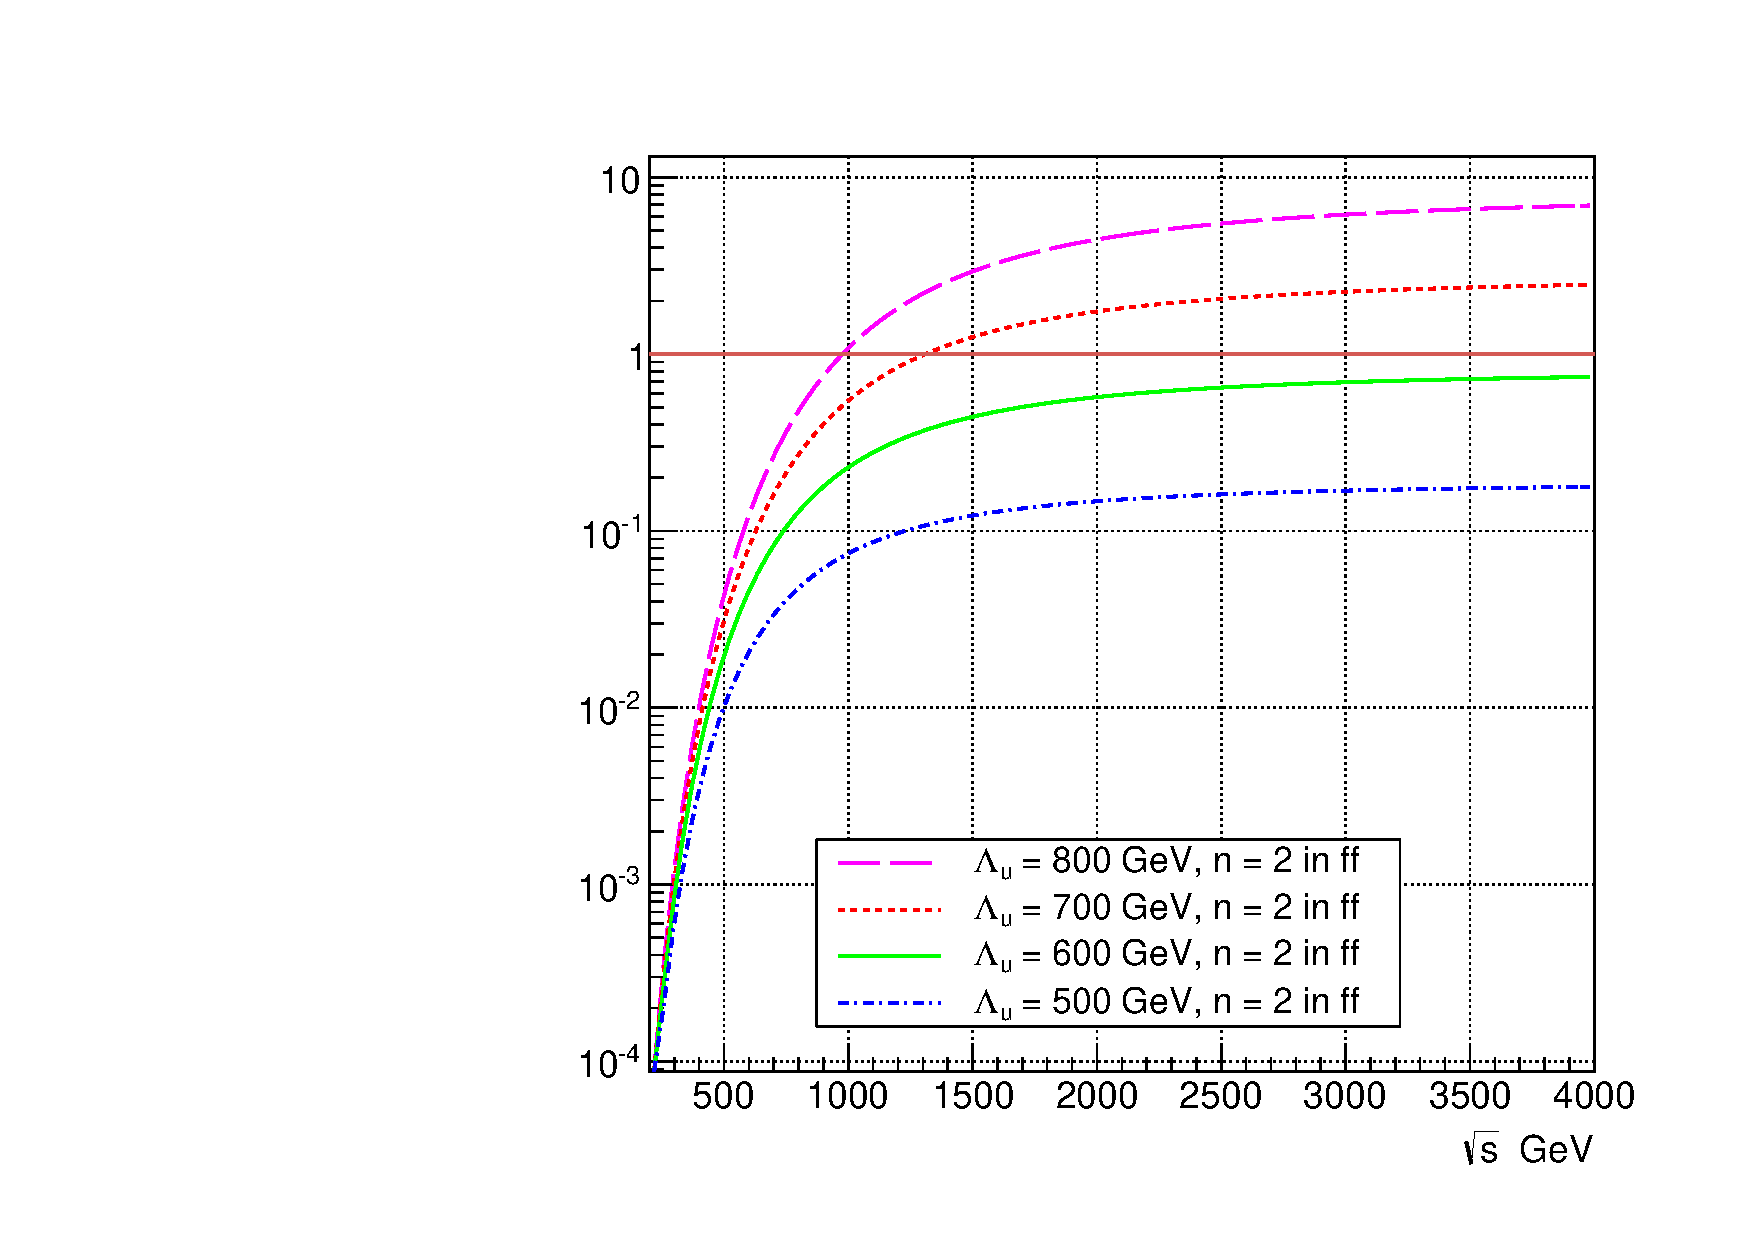
\includegraphics[width=0.4\textwidth]{figs/unitarity.pdf}
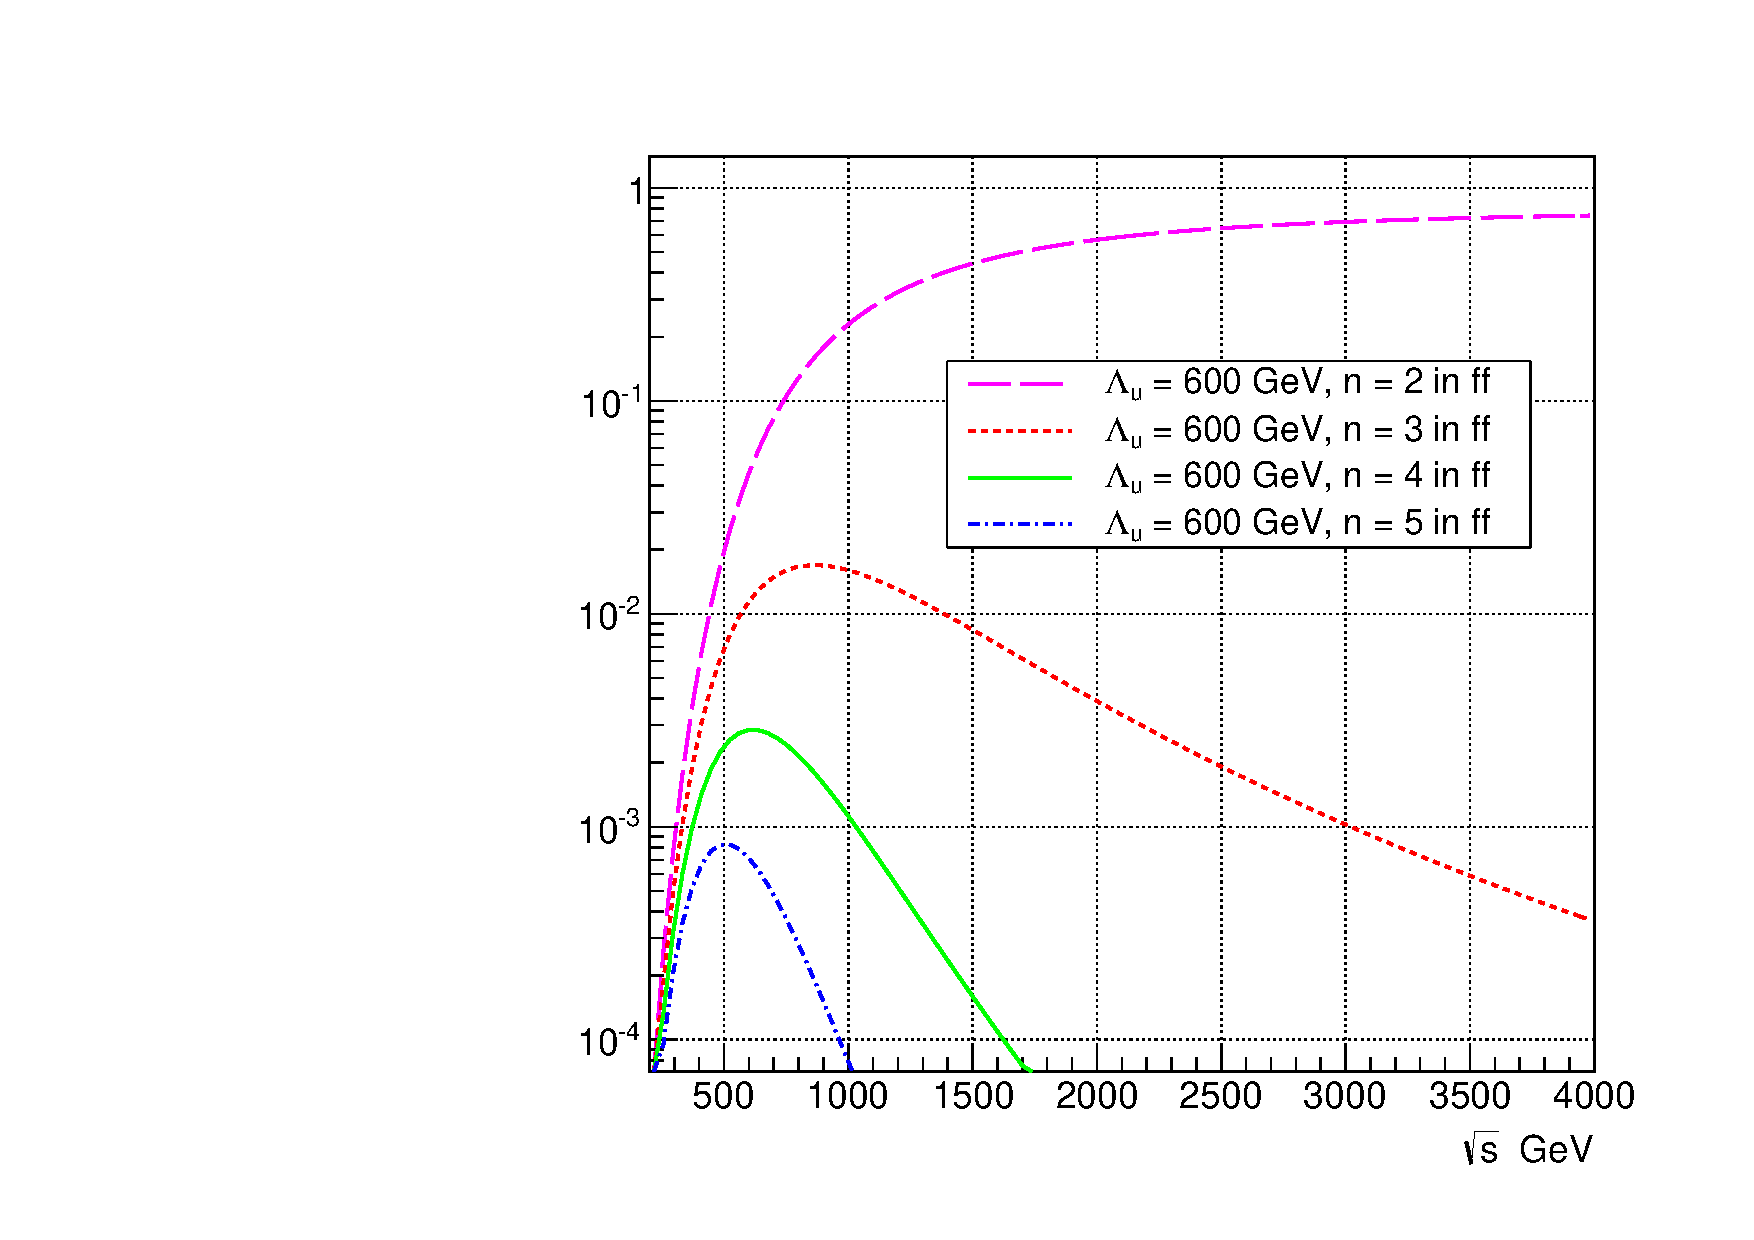
\includegraphics[width=0.4\textwidth]{figs/unitarity_n.pdf}
\caption{\label{aqgc:unitarity} The unitarity condition for aQGC $a_0^W/\Lambda^2 = 1\times 10^{-4}$~GeV$^{-2}$, the unitarity bound is represented by the line of value 1 }}
\end{figure}

We also have examined the unitarity condition for aQGC parameters as a function of the form factor scale $\Lambda_{u}$ and different values of $\hat{s}$, and compared it with the projected
sensitivity of our analysis using 20~\fbinv of integrated luminosity. To do this, we fixed the value of $aQGC \times ff$ to the value of $aQGC$ without a form factor. The center of mass energy dependence is replaced with a fixed effective energy scale representing the typical center of mass energy with non-zero value of a aQGC. In our analysis, we have used the limits with a form factor in Eq.~\ref{aqgc:ff}, which is the same as former CMS analysis on two photon production of W boson pair ~\cite{CMS-PAS-FSQ-12-010}, to fix this effective $\sqrt{\hat{s}}$. In this way, we can vary the value of the effective $\sqrt{\hat{s}}$ to estimate uncertainties of our limits. In Figure ~\ref{aqgc:uniBand} uncertainty bands with 0.5/2, 0.25/4 times the effective $\sqrt{\hat{s}}$ are shown. Besides, we have also drawn theoretical unitarity bound with different $\sqrt{\hat{s}}$ upper limits. The results shown on Figure ~\ref{aqgc:uniBand} indicates that there is no value of the dipole form factor's scale at
which the unitarity condition can be satisfied for all values of
$WW\gamma$ invariant mass, given the available amount of data at
$\sqrt{s}=8$~TeV. This motivates the choice of presenting our results
without any form factor.

\begin{figure}[hb] 
  \begin{center}
    \subfigure[$a_0^W$]{
    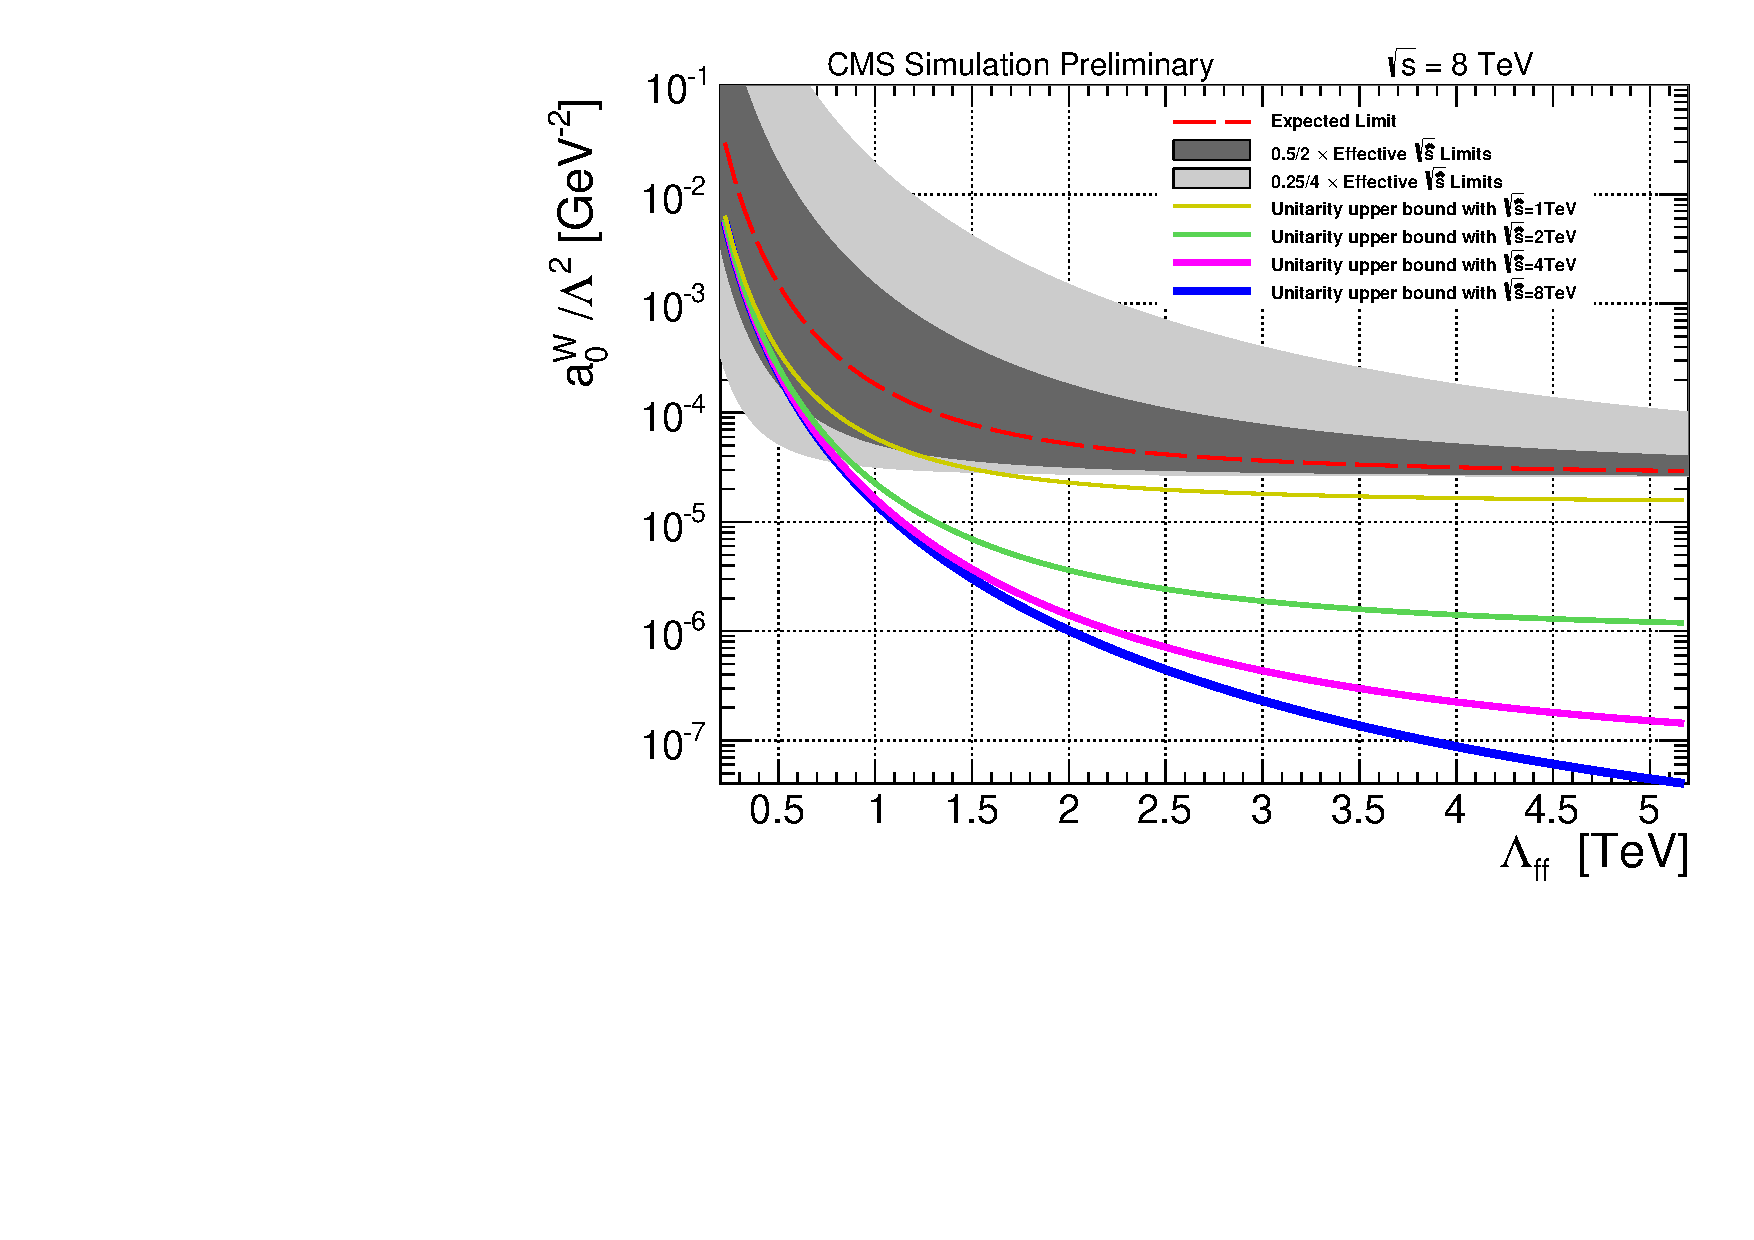
\includegraphics[width=0.48\textwidth]{figs/prounitarity_a0w.pdf}
    }
    \subfigure[$a_C^W$]{
    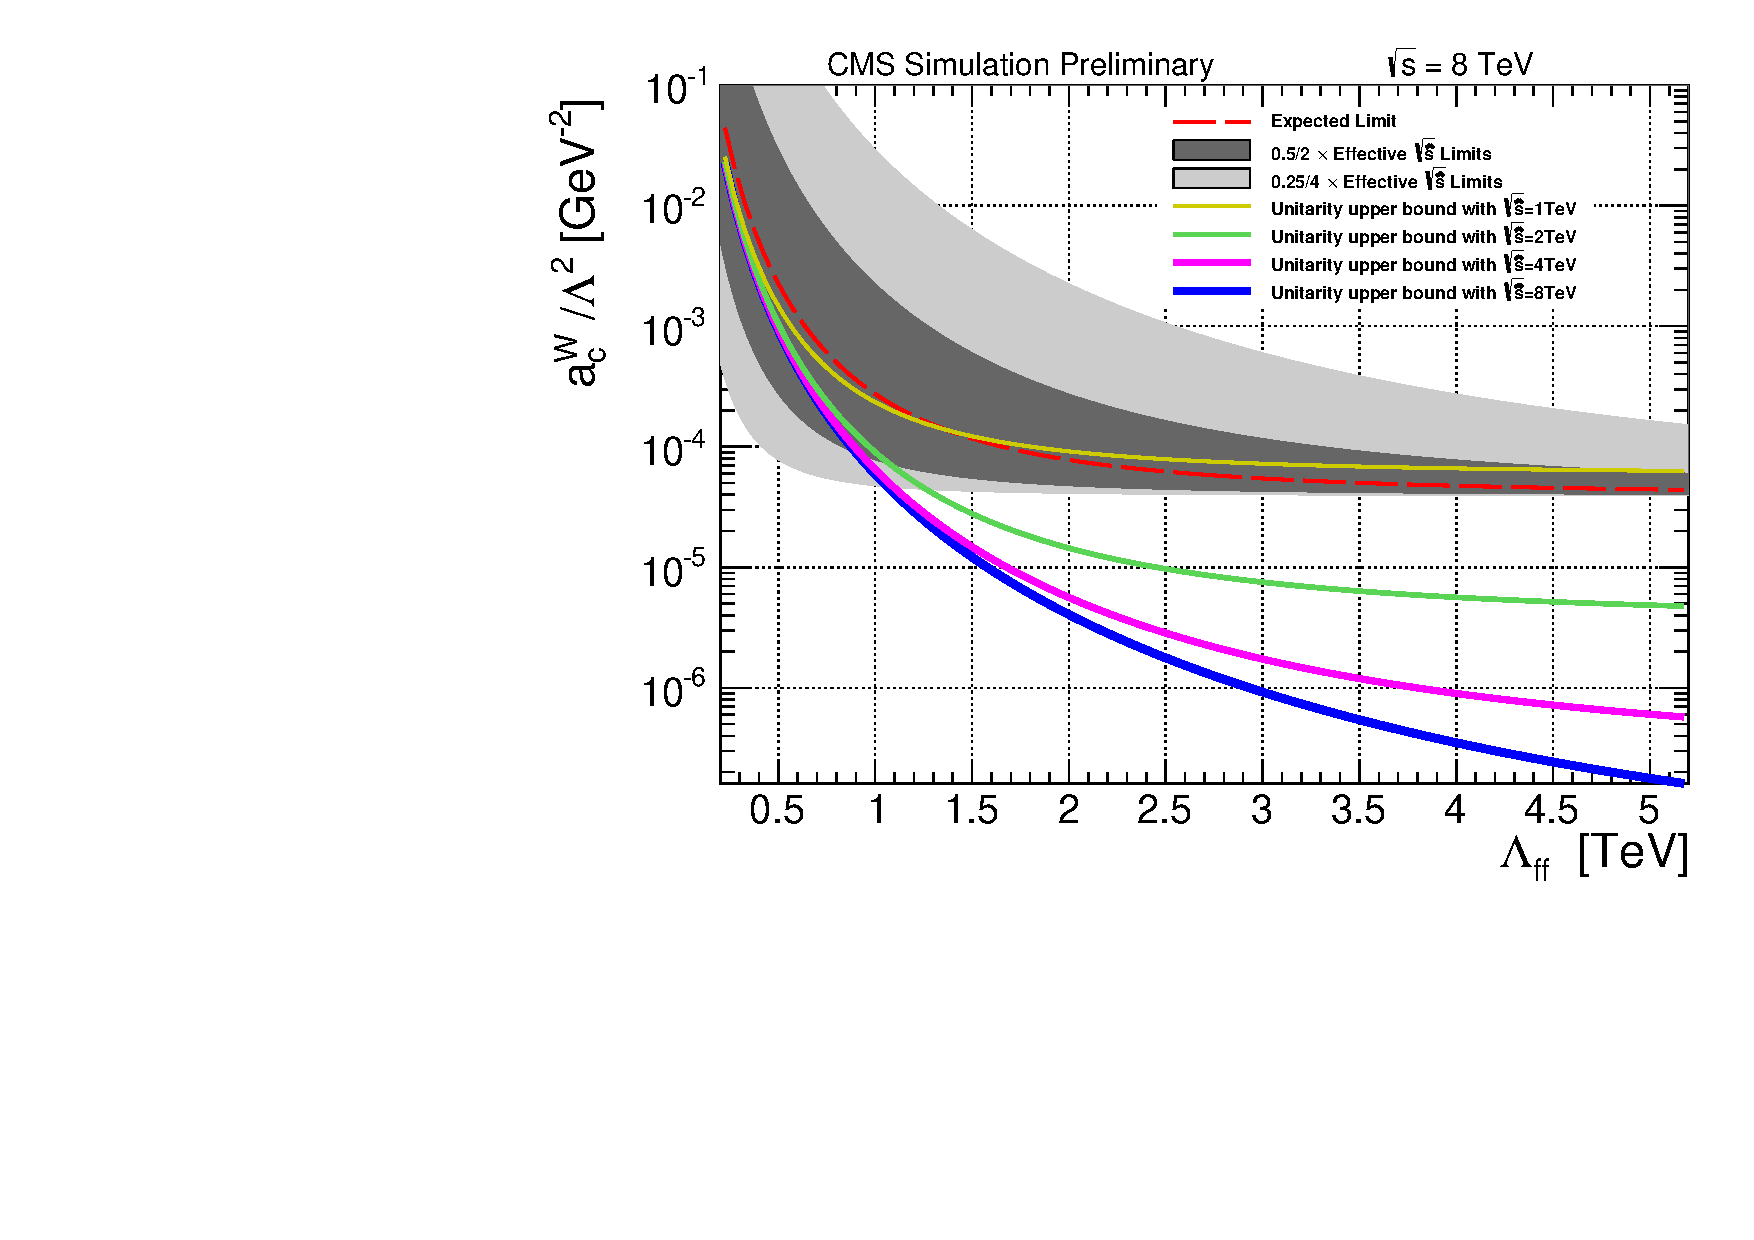
\includegraphics[width=0.48\textwidth]{figs/prounitarity_acw.pdf}
    }\\
    \subfigure[$\kappa_0^W$]{
    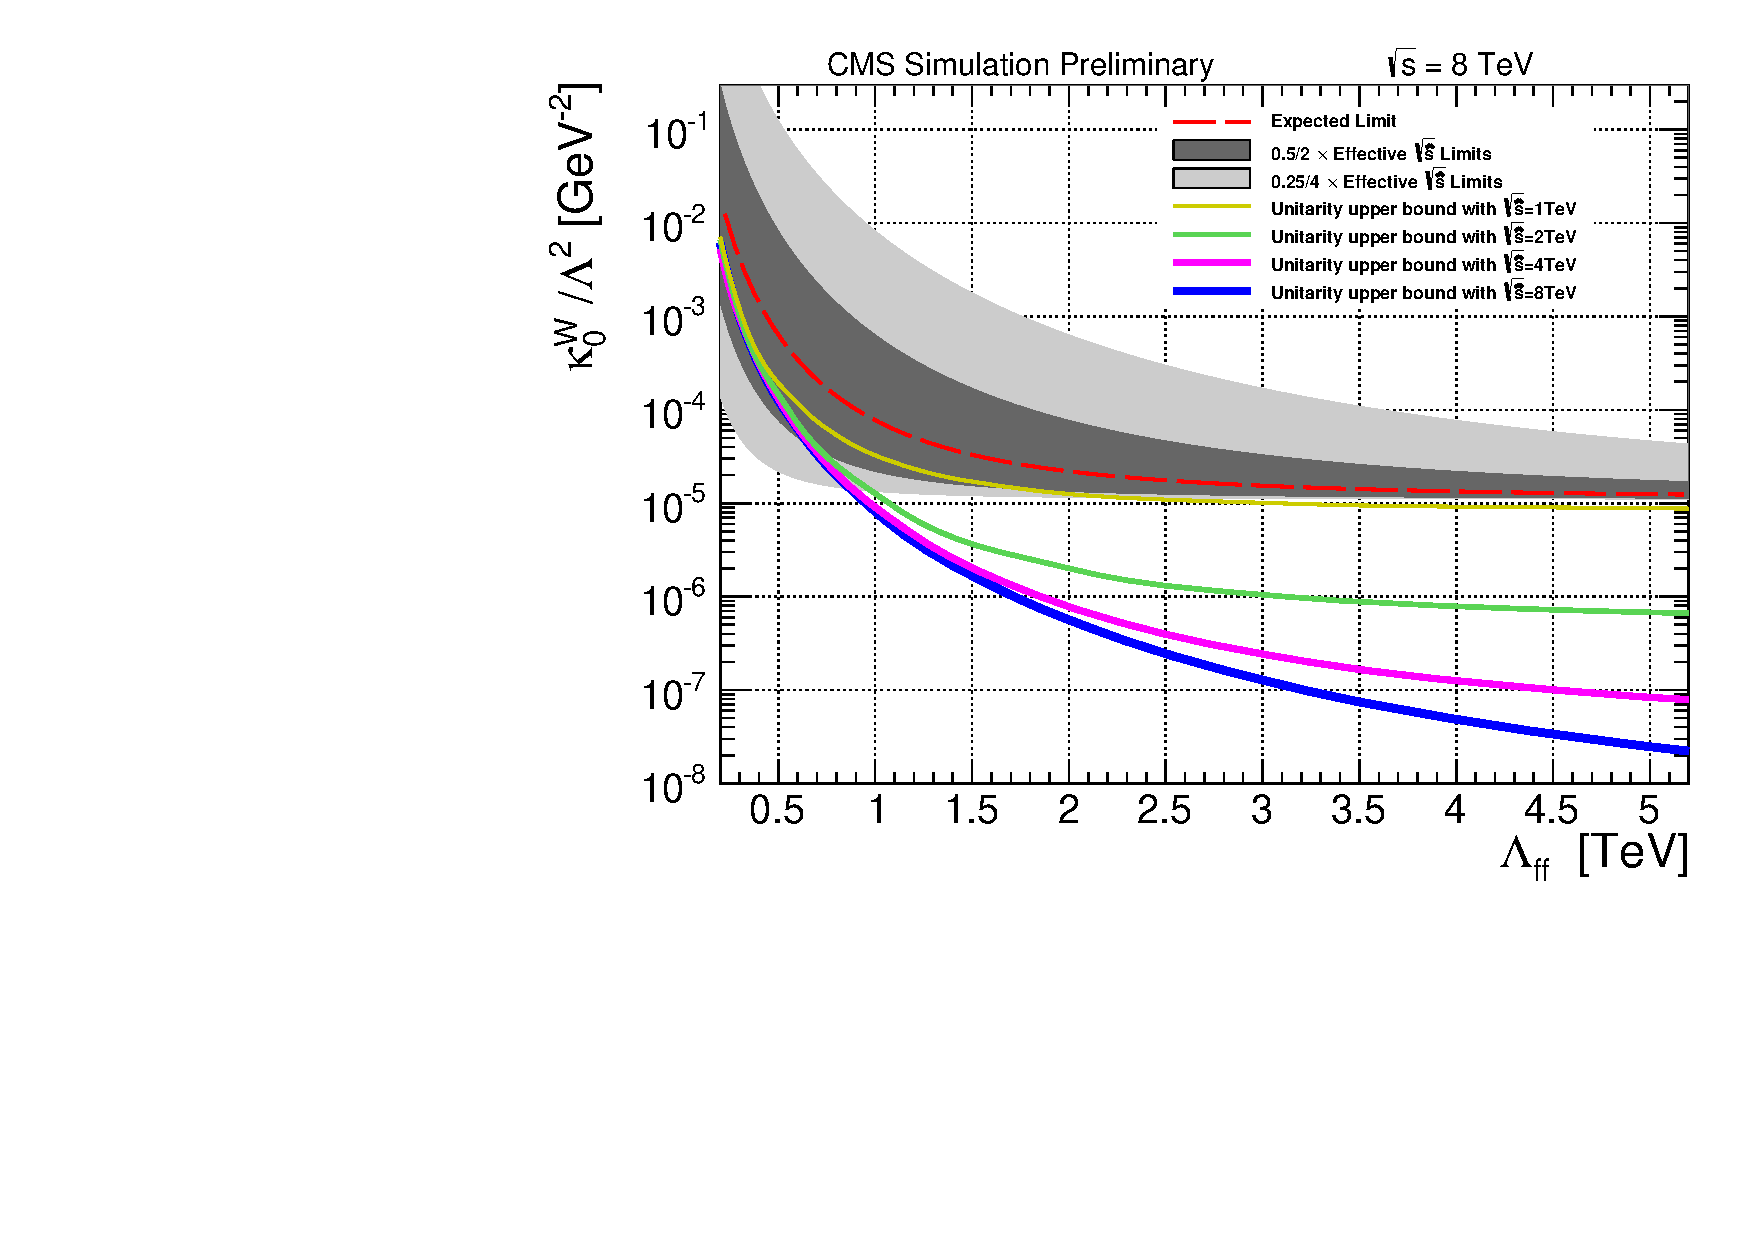
\includegraphics[width=0.48\textwidth]{figs/prounitarity_k0W.pdf}
    }
    \subfigure[$\kappa_C^W$]{
    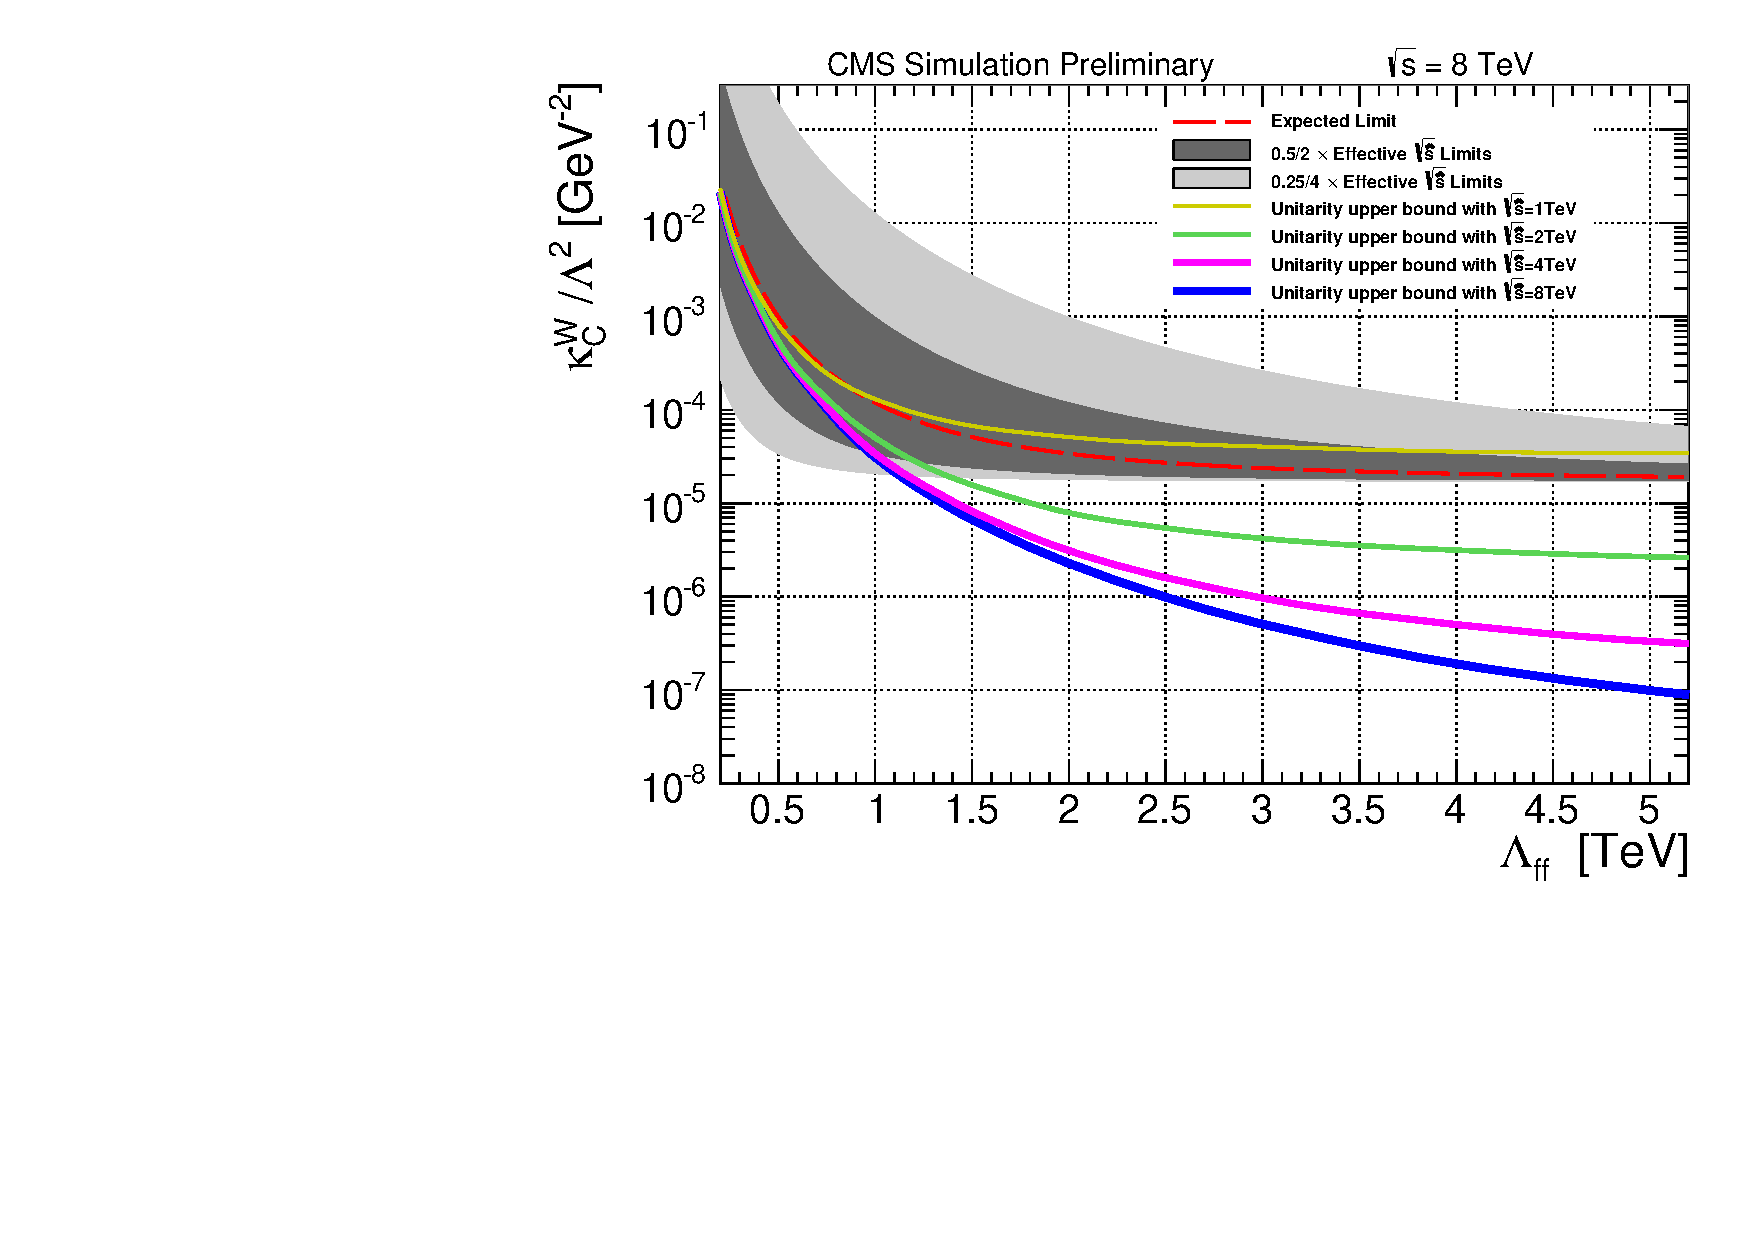
\includegraphics[width=0.48\textwidth]{figs/prounitarity_kCW.pdf}
    }\\
    \subfigure[$f_{T,0}$]{
    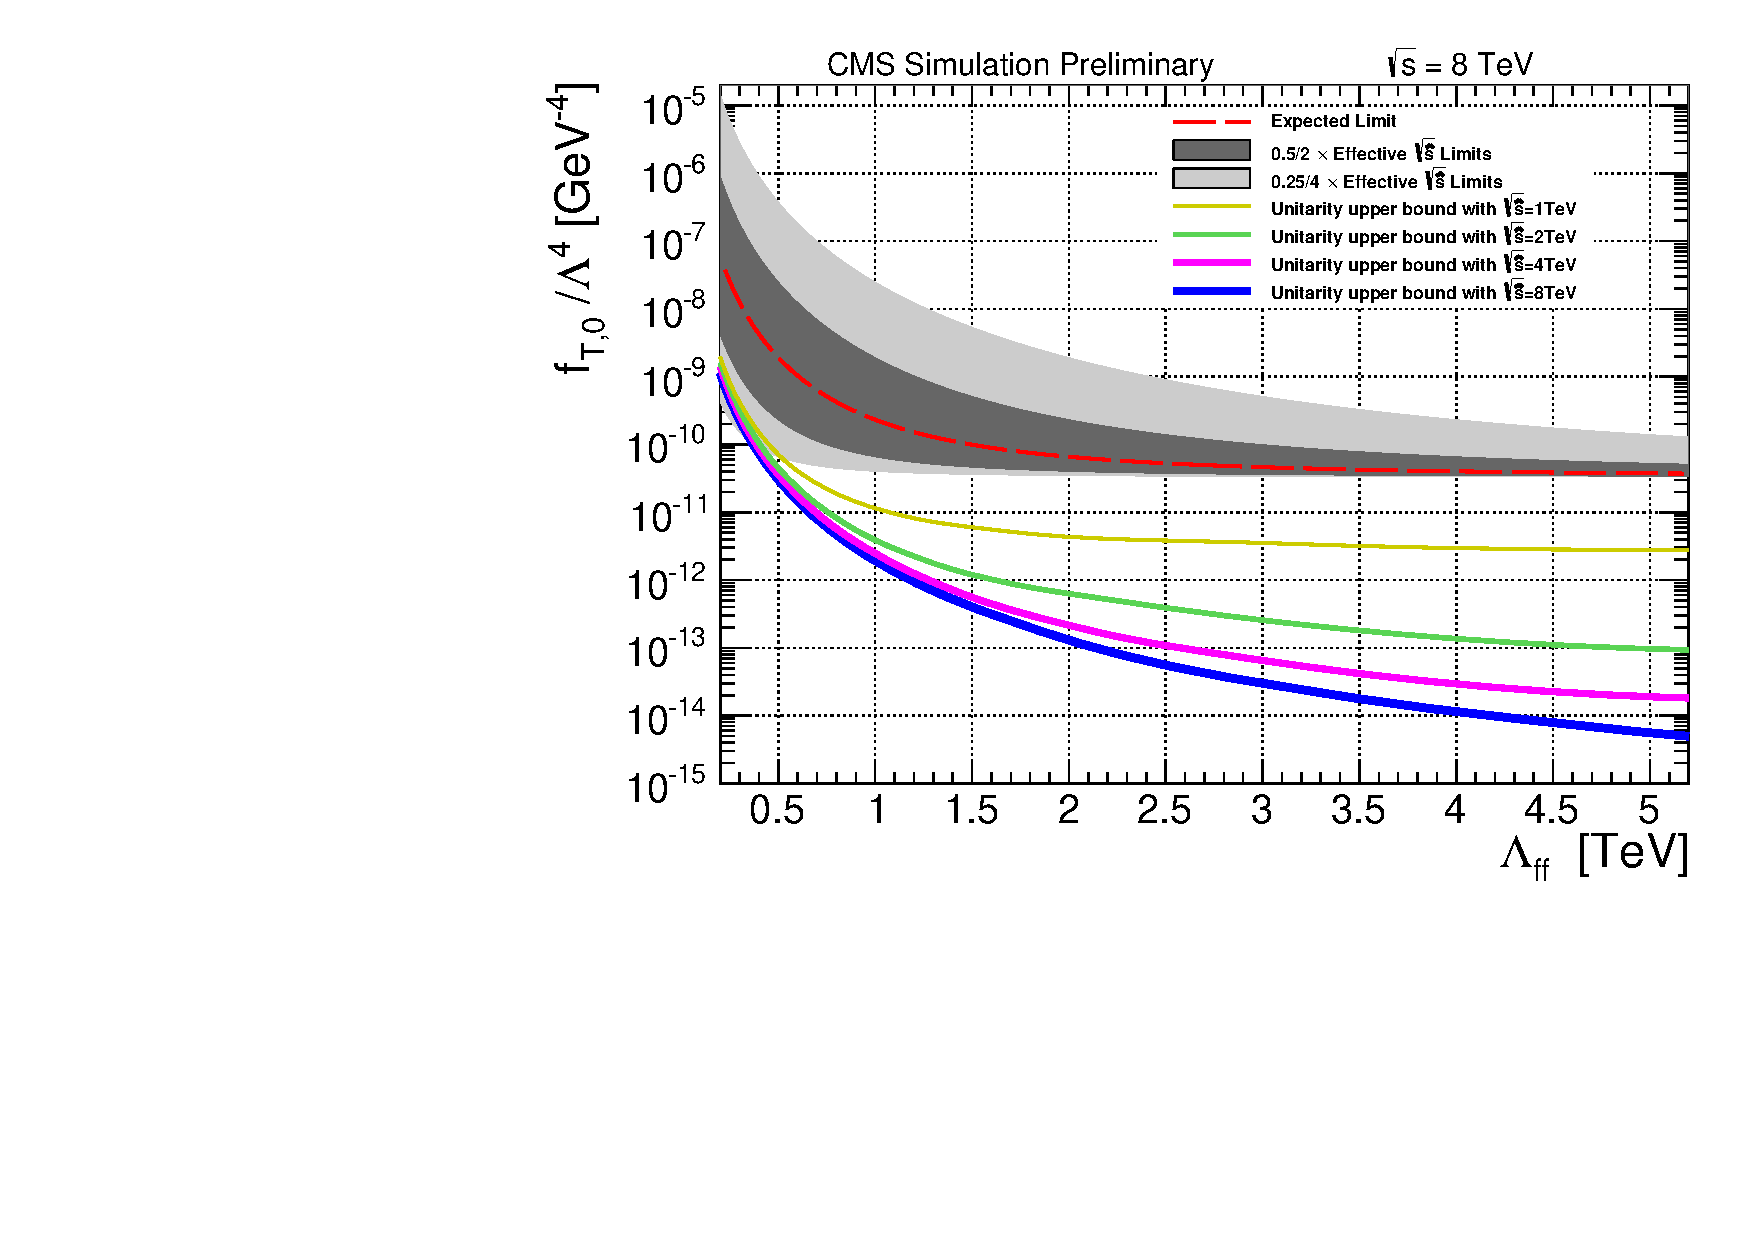
\includegraphics[width=0.48\textwidth]{figs/prounitarity_fT0.pdf}
    }
    \caption{\label{aqgc:uniBand} The unitarity condition for aQGC
    parameters (a) $a_0^W/\Lambda^2$, (b) $a_{C}^{W}/\Lambda^{2}$, (c) $\kappa_0^W/\Lambda^2$, (d) $\kappa_{C}^{W}/\Lambda^{2}$ and
    (e) $f_{T,0}/\Lambda^{4}$ as a function of form factor parameter
    $\Lambda_{u}$ and different values of $\hat{s}$ is compared with
    the projected sensitivity of our analysis using 20~\fbinv of integrated
    luminosity. }
  \end{center}
\end{figure}
\clearpage
